%%%%%%%%%%%%%%%%%%%%%%%%%%%%%%%%%%%%%%%%%
% Beamer Presentation
% LaTeX Template
% Version 1.0 (10/11/12)
%
% This template has been downloaded from:
% http://www.LaTeXTemplates.com
%
% License:
% CC BY-NC-SA 3.0 (http://creativecommons.org/licenses/by-nc-sa/3.0/)
%
%%%%%%%%%%%%%%%%%%%%%%%%%%%%%%%%%%%%%%%%%

%----------------------------------------------------------------------------------------
%	PACKAGES AND THEMES
%----------------------------------------------------------------------------------------

\documentclass[aspectratio=169]{beamer}
%\documentclass{beamer}

\mode<presentation> {

% The Beamer class comes with a number of default slide themes
% which change the colors and layouts of slides. Below this is a list
% of all the themes, uncomment each in turn to see what they look like.

%\usetheme{default}
%\usetheme{AnnArbor}
%\usetheme{Antibes}
%\usetheme{Bergen}
%\usetheme{Berkeley}
%\usetheme{Berlin}
%\usetheme{Boadilla}
%\usetheme{CambridgeUS}
%\usetheme{Copenhagen}
%\usetheme{Darmstadt}
%\usetheme{Dresden}
%\usetheme{Frankfurt}
%\usetheme{Goettingen}
%\usetheme{Hannover}
%\usetheme{Ilmenau}
%\usetheme{JuanLesPins}
%\usetheme{Luebeck}
\usetheme{Madrid}
%\usetheme{Malmoe}
%\usetheme{Marburg}
%\usetheme{Montpellier}
%\usetheme{PaloAlto}
%\usetheme{Pittsburgh}
%\usetheme{Rochester}
%\usetheme{Singapore}
%\usetheme{Szeged}
%\usetheme{Warsaw}

% As well as themes, the Beamer class has a number of color themes
% for any slide theme. Uncomment each of these in turn to see how it
% changes the colors of your current slide theme.

%\usecolortheme{albatross}
%\usecolortheme{beaver}
%\usecolortheme{beetle}
%\usecolortheme{crane}
%\usecolortheme{dolphin}
%\usecolortheme{dove}
%\usecolortheme{fly}
%\usecolortheme{lily}
%\usecolortheme{orchid}
%\usecolortheme{rose}
%\usecolortheme{seagull}
%\usecolortheme{seahorse}
%\usecolortheme{whale}
%\usecolortheme{wolverine}

%\setbeamertemplate{footline} % To remove the footer line in all slides uncomment this line
%\setbeamertemplate{footline}[page number] % To replace the footer line in all slides with a simple slide count uncomment this line

%\setbeamertemplate{navigation symbols}{} % To remove the navigation symbols from the bottom of all slides uncomment this line
}

\usepackage{graphicx} % Allows including images
\usepackage{booktabs} % Allows the use of \toprule, \midrule and \bottomrule in tables
%\RequirePackage{beamerthemeoracle}

%----------------------------------------------------------------------------------------
%	TITLE PAGE
%----------------------------------------------------------------------------------------

\title[Introduction to Oracle VM (Xen) Networking]{Introduction to Oracle VM (Xen) Networking} % The short title appears at the bottom of every slide, the full title is only on the title page

\author{Dongli Zhang} % Your name
\institute[Oracle] % Your institution as it will appear on the bottom of every slide, may be shorthand to save space
{
Oracle Asia Research and Development Centers (Beijing) \\ % Your institution for the title page
\medskip
\textit{dongli.zhang@oracle.com} % Your email address
}
\date{\today} % Date, can be changed to a custom date

\begin{document}

%------------------------------------------------

\section{Title}
\begin{frame}
\titlepage % Print the title page as the first slide
\end{frame}

%------------------------------------------------

\section{Plan}
\begin{frame}
\frametitle{Plan}
\begin{itemize}
\setlength\itemsep{1em}
\item {\large Paravirtualized Networking}
	\begin{itemize}
		\item vif, bridge, bond
	\end{itemize}
\item {\large Emulated Networking}
\item {\large Environment:}
	\begin{itemize}
		\item xen: Oracle VM server 3.3.3 with xen-4.3.0-55.el6.47.33.x86\_64
		\item dom0: Unbreakable Enterprise Kernel v4.1.12-89
		\item domU: Unbreakable Enterprise Kernel v4.1.12-89
	\end{itemize}
\item Prerequisite Knowledge: http://finallyjustice.github.io/xen-arch.pdf
	\begin{itemize}
		\item xen framework
		\item PVM vs. HVM vs. PVHVM
		\item event channel, grant table
		\item xen admin hands-on experience (preferred)
	\end{itemize}
\end{itemize}
\end{frame}

%------------------------------------------------

\section{Paravirtualized xen-netfront/xen-netback framework}
\begin{frame}
\frametitle{Paravirtual xen-netfront/xen-netback framework}
\begin{figure}
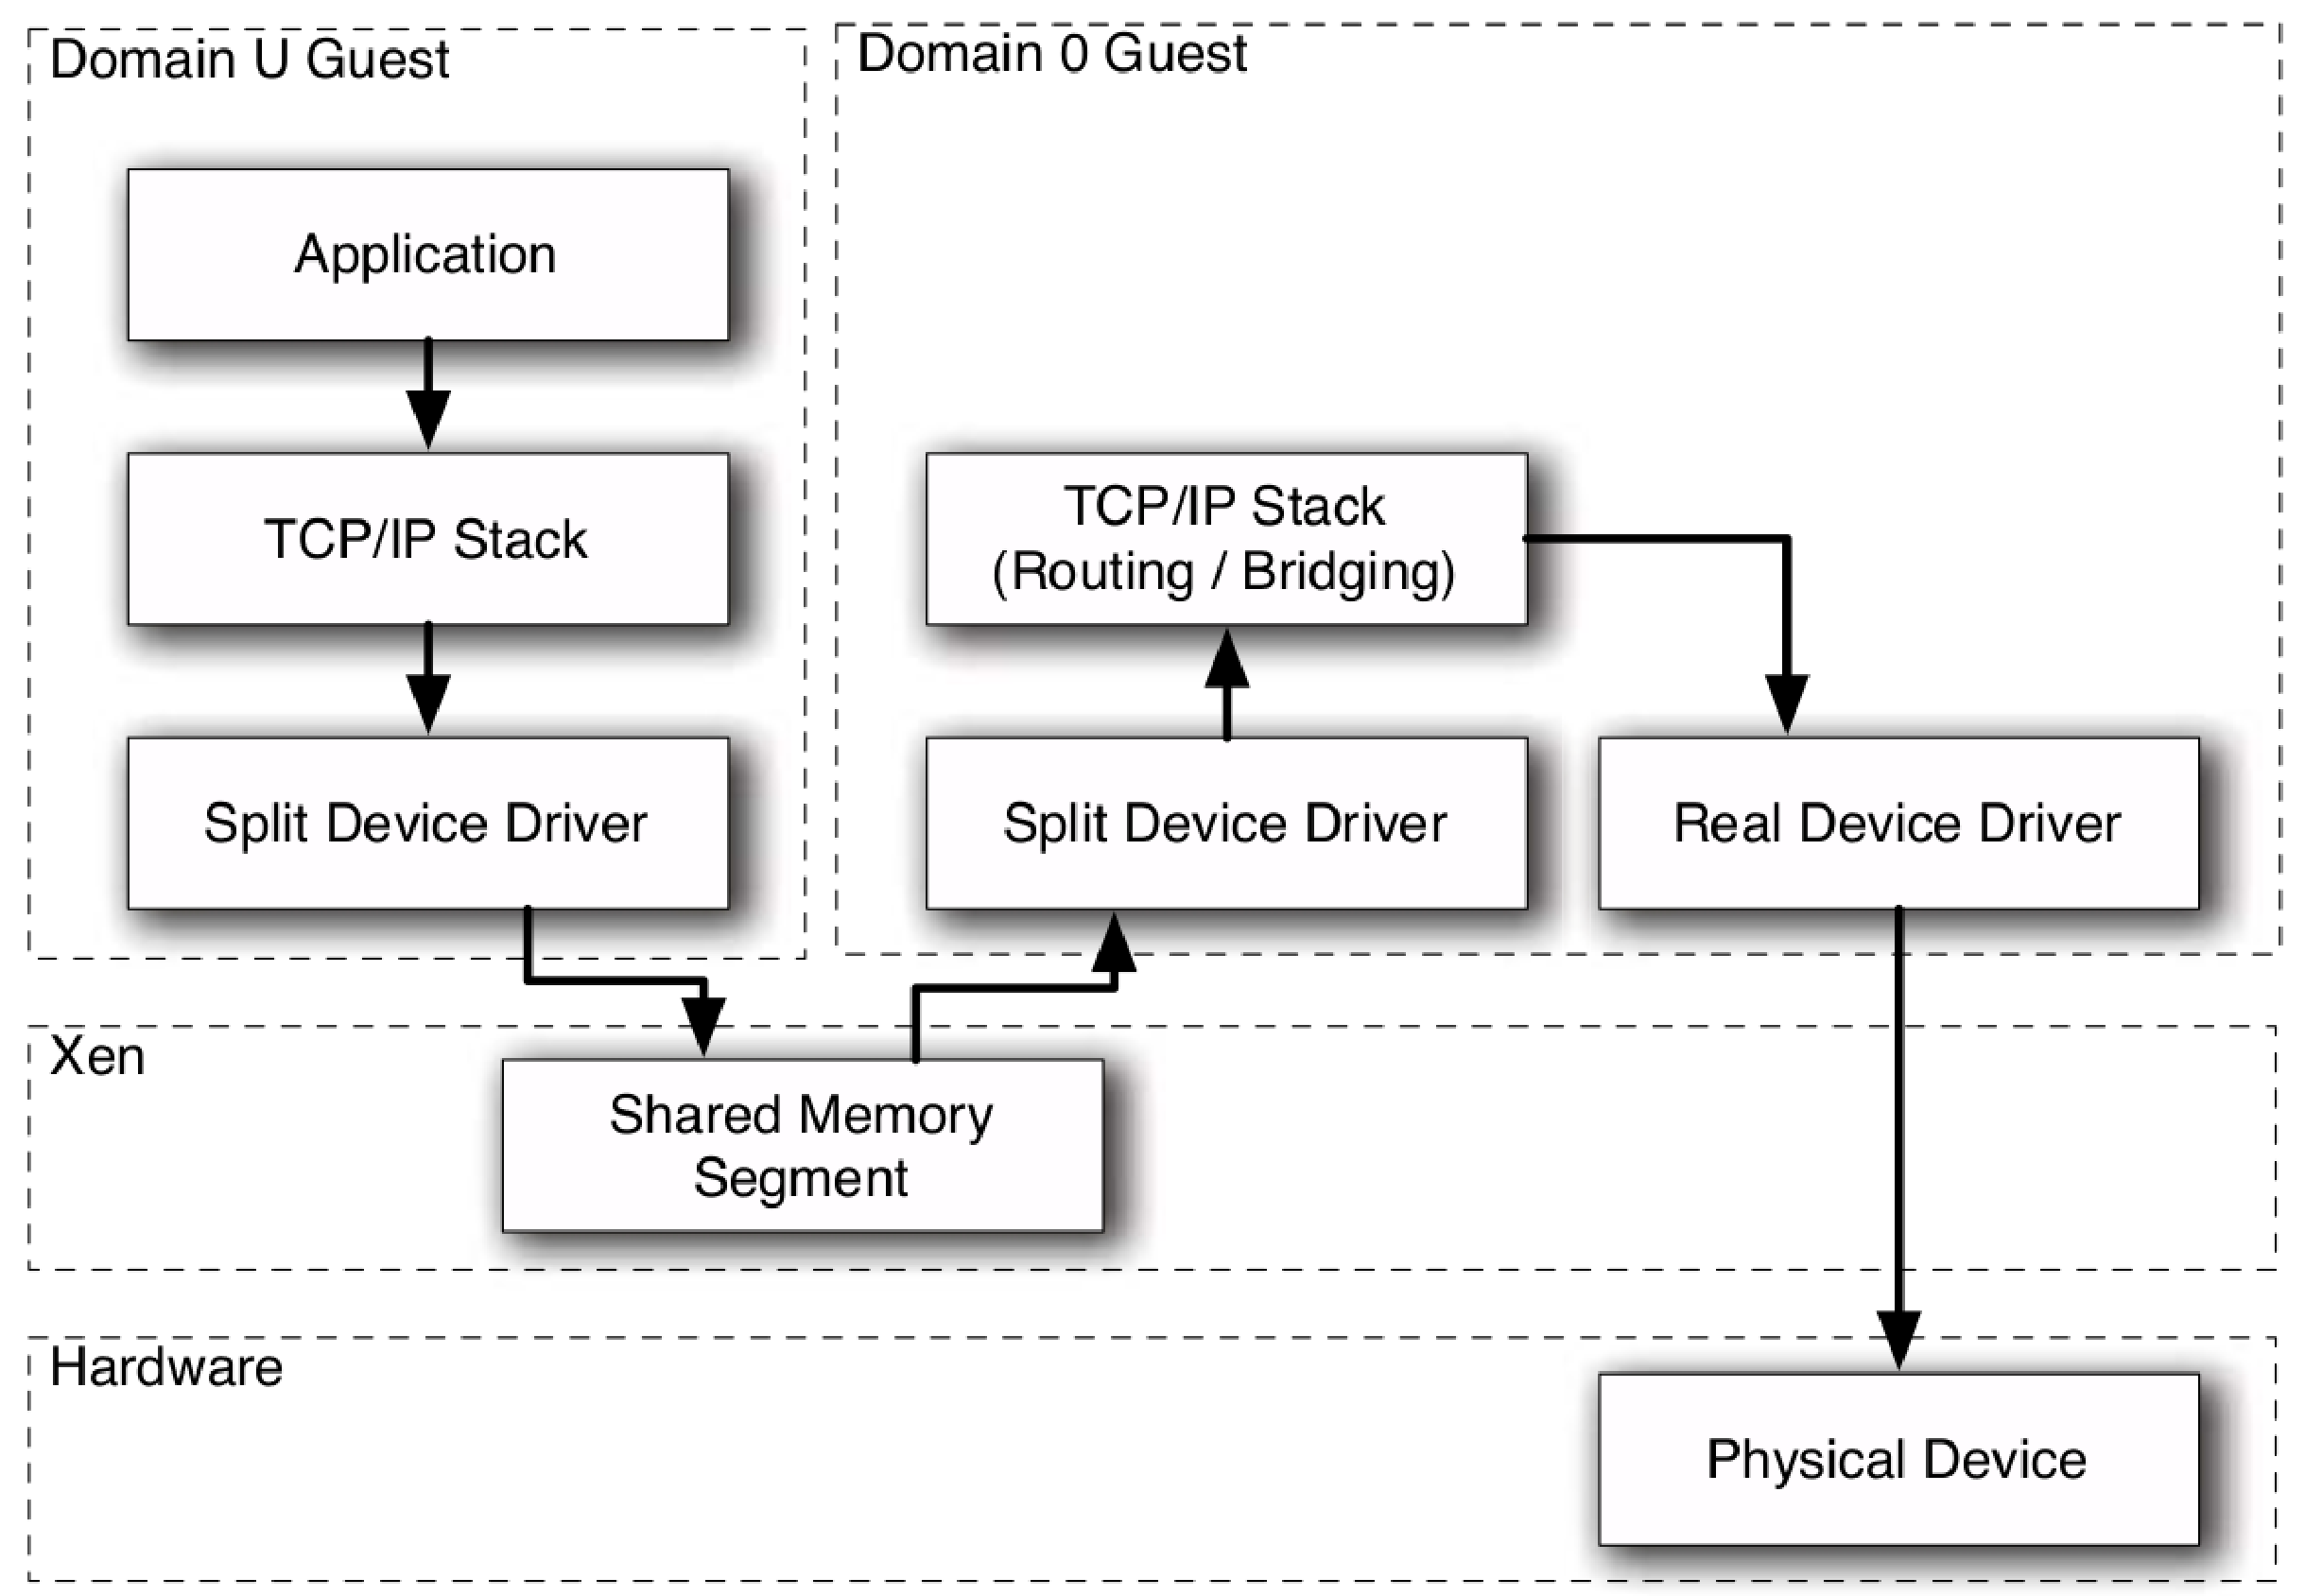
\includegraphics[width=0.7\linewidth]{figures/xennet1.pdf}
\end{figure}
\end{frame}

%------------------------------------------------

\section{xen-netfront/xen-netback source code}
\begin{frame}
\frametitle{xen-netfront/xen-netback source code}
\begin{block}{Unbreakable Enterprise Kernel v4.1.12-89}
\begin{itemize}
\item drivers/net/xen-netfront.c
\item drivers/net/xen-netback/xenbus.c
\item drivers/net/xen-netback/netback.c
\item drivers/net/xen-netback/interface.c
\end{itemize}
\end{block}
\frametitle{xen-netfront/xen-netback source code}
\begin{block}{kernel upstream v4.9-rc8}
\begin{itemize}
\item drivers/net/xen-netfront.c
\item drivers/net/xen-netback/xenbus.c
\item drivers/net/xen-netback/netback.c
\item drivers/net/xen-netback/interface.c
\item drivers/net/xen-netback/rx.c
\item drivers/net/xen-netback/hash.c
\end{itemize}
\end{block}
\end{frame}

%------------------------------------------------

\section{Paravirtualized networking scenario 1/2}
\begin{frame}
\frametitle{Paravirtual networking scenario 1/2}
\begin{figure}
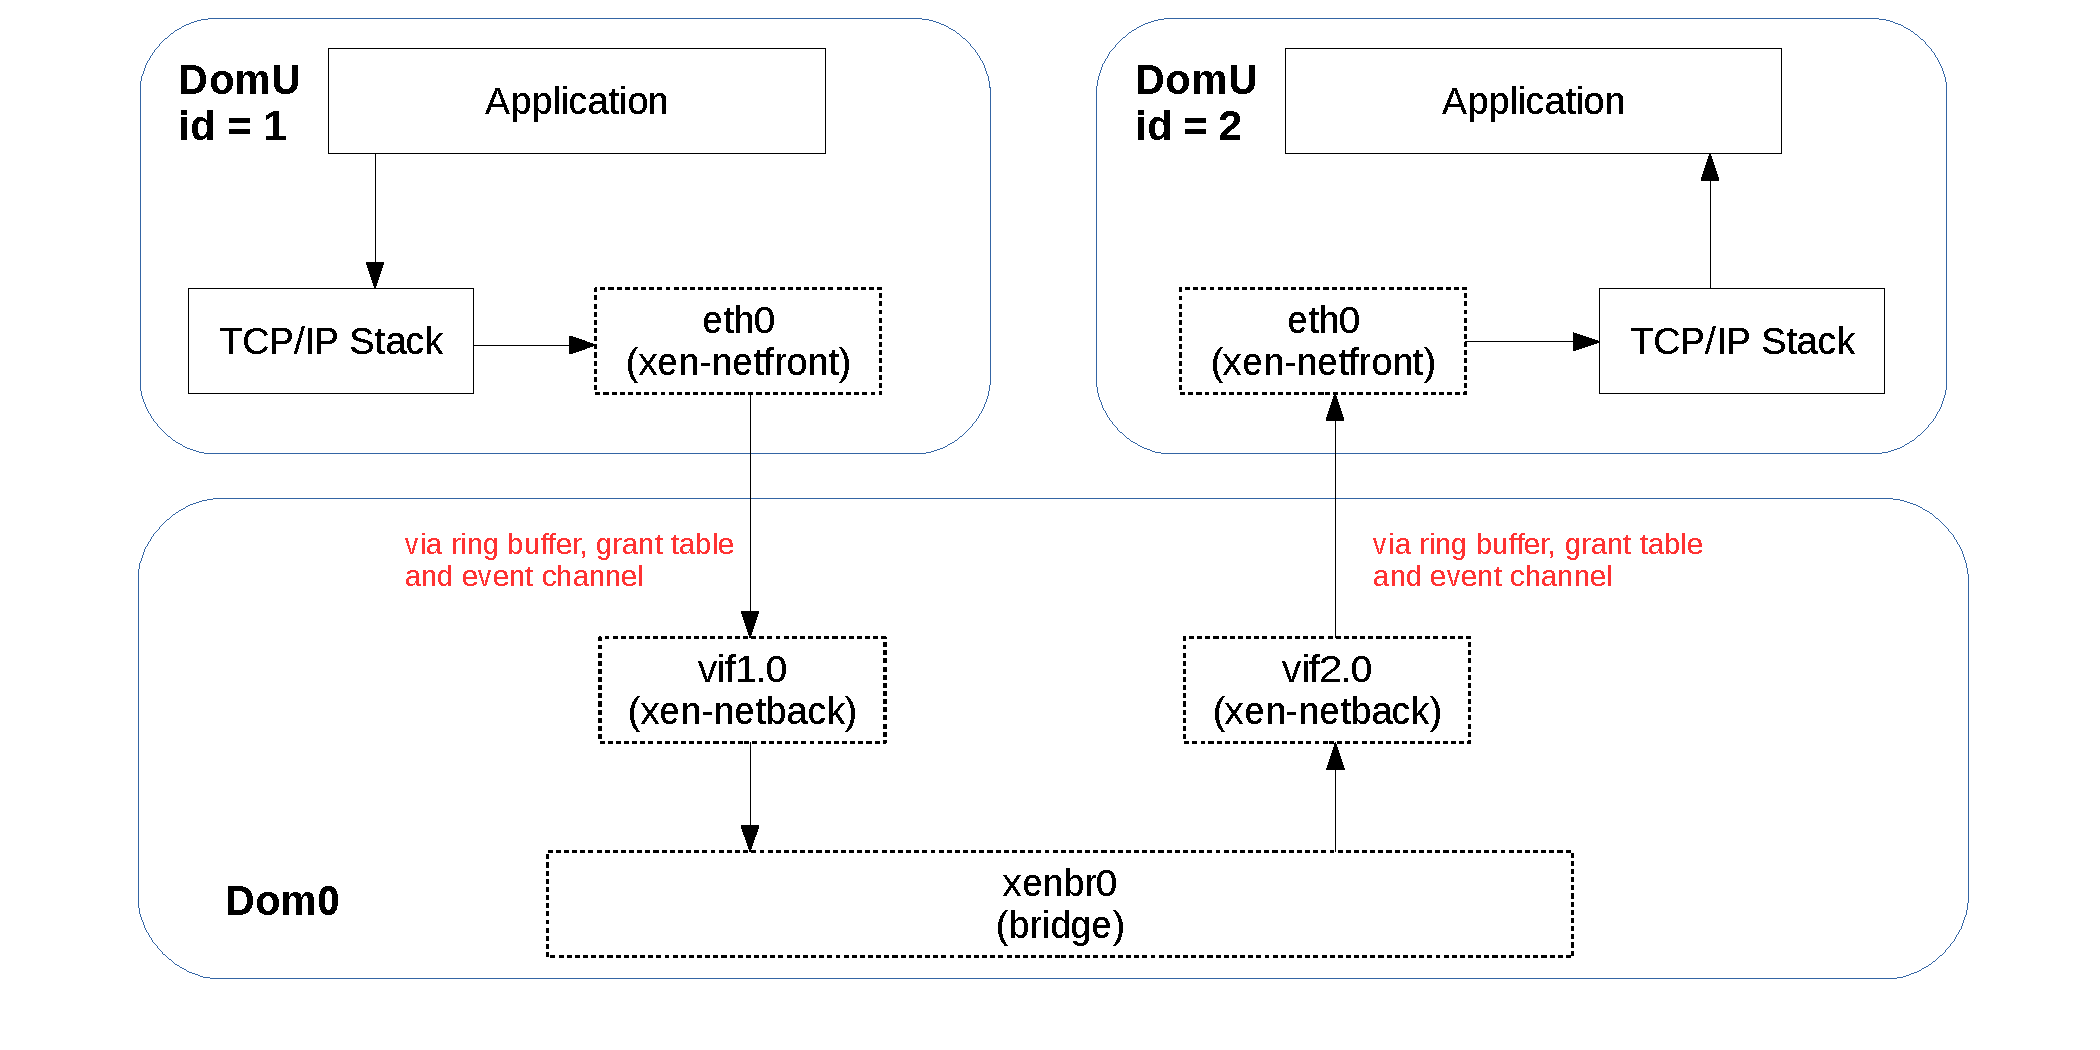
\includegraphics[width=1.0\linewidth]{figures/xennet2.pdf}
\end{figure}
\end{frame}

%------------------------------------------------

\section{Paravirtualized networking scenario 2/2}
\begin{frame}
\frametitle{Paravirtual networking scenario 2/2}
\begin{figure}
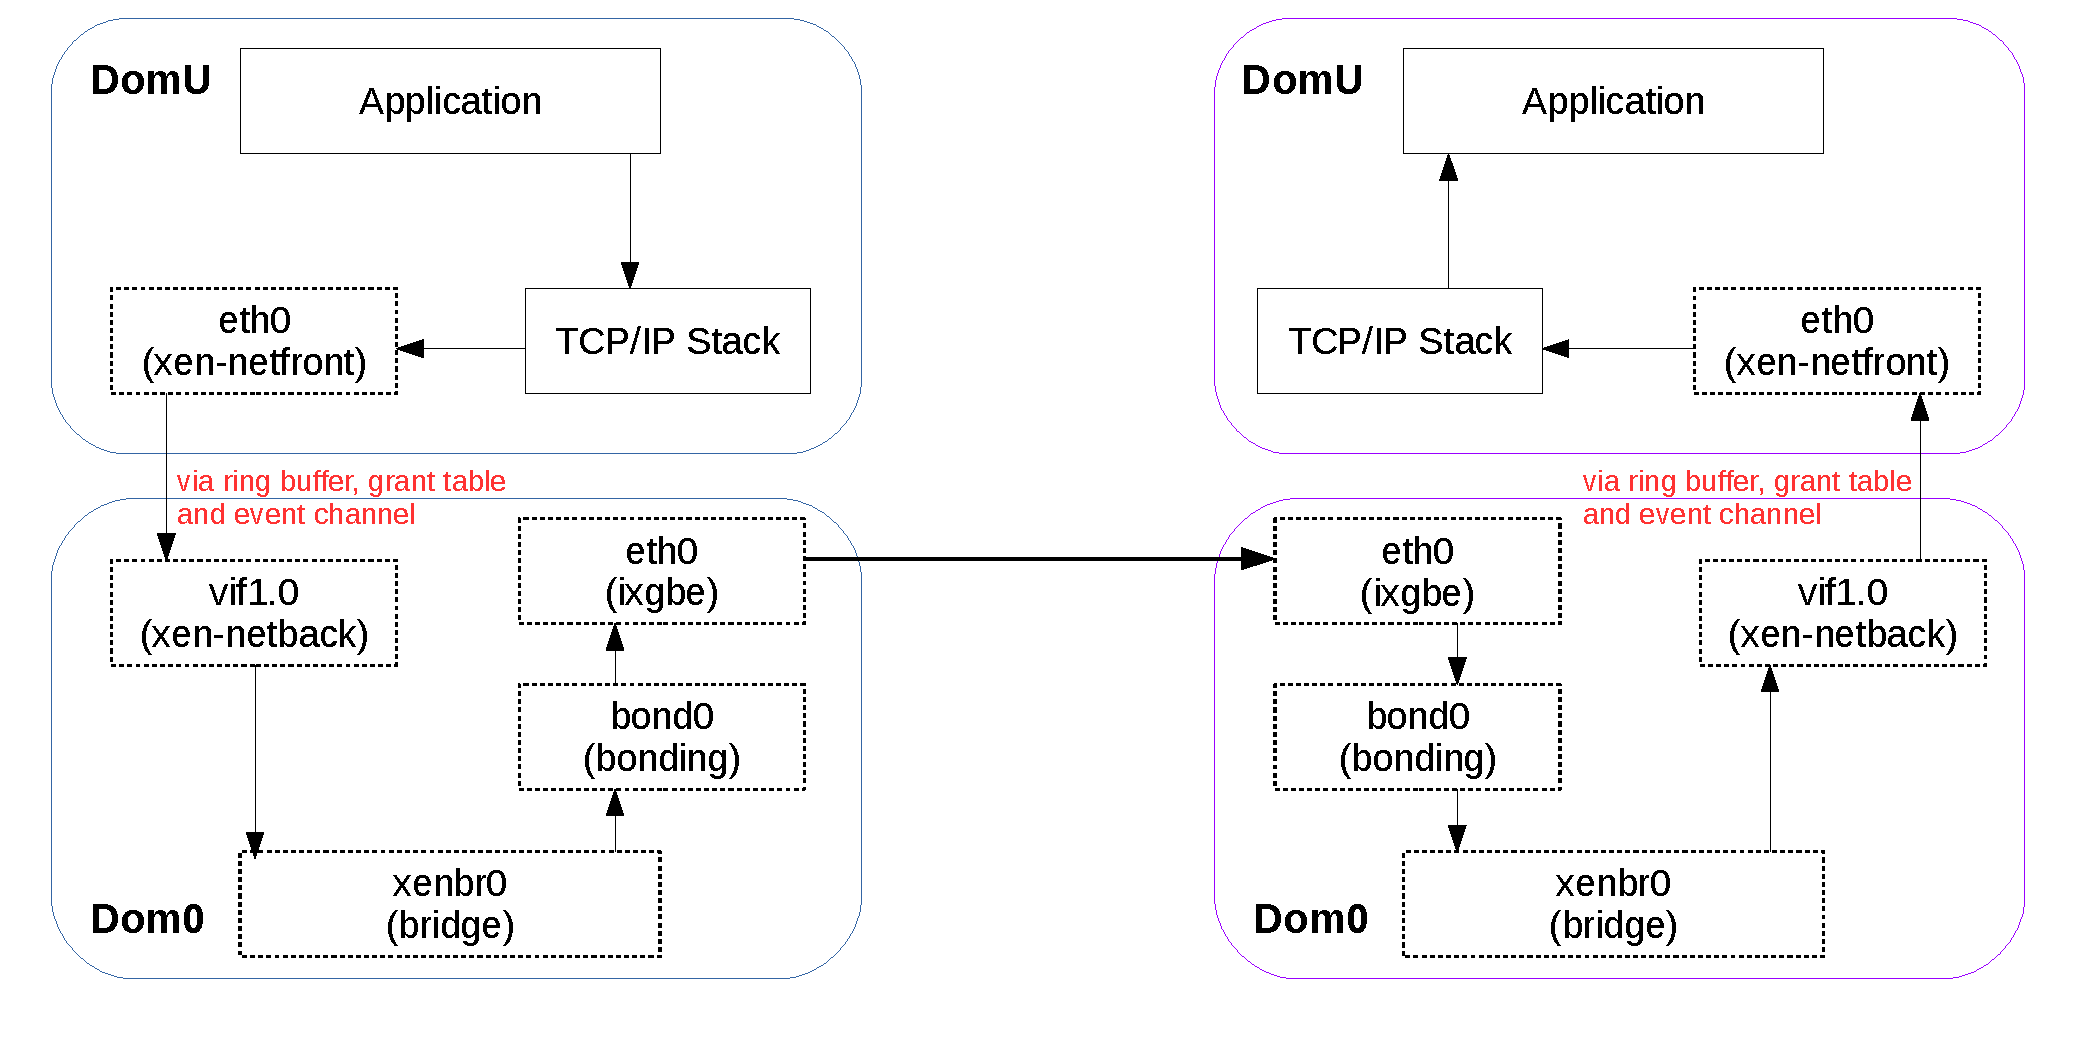
\includegraphics[width=1.0\linewidth]{figures/xennet3.pdf}
\end{figure}
\end{frame}

%------------------------------------------------

\section{PV driver vs. PCI driver}
\begin{frame}
\frametitle{PV driver vs. PCI driver}
\begin{table}
\begin{tabular}{l l l}
\toprule
& \textbf{PCI driver} & \textbf{PV driver}\\
\midrule
\textbf{device abstraction} & \textcolor{blue}{pci\_device, pci\_driver} & \visible<2->{\textcolor{red}{xenbus\_device, xenbus\_driver}} \\
\textbf{device discovery} & \textcolor{blue}{PCI Tree} & \visible<3->{\textcolor{red}{Xenstore}} \\
\textbf{device configuration} & \textcolor{blue}{PCI Config Space (IO/MMIO)} & \visible<4->{\textcolor{red}{Xenstore}} \\
\textbf{data flow} & \textcolor{blue}{DMA Ring Buffer} & \visible<5->{\textcolor{red}{Memory Ring Buffer}} \\
\textbf{shared memory} & \textcolor{blue}{N/A or IOMMU} & \visible<6->{\textcolor{red}{Grant Table}} \\
\textbf{interrupt} & \textcolor{blue}{IOAPIC, MSI, MSI-X} & \visible<7->{\textcolor{red}{Event Channel}} \\
\bottomrule
\end{tabular}
\end{table}
\begin{figure}

\includegraphics[width=.24\linewidth]{figures/fight.pdf}
\end{figure}
\end{frame}

%------------------------------------------------

\section{pv xmit: front ---> backend 1/3}
\begin{frame}
\frametitle{pv xmit: front ---$>$ backend 1/3}
\begin{figure}
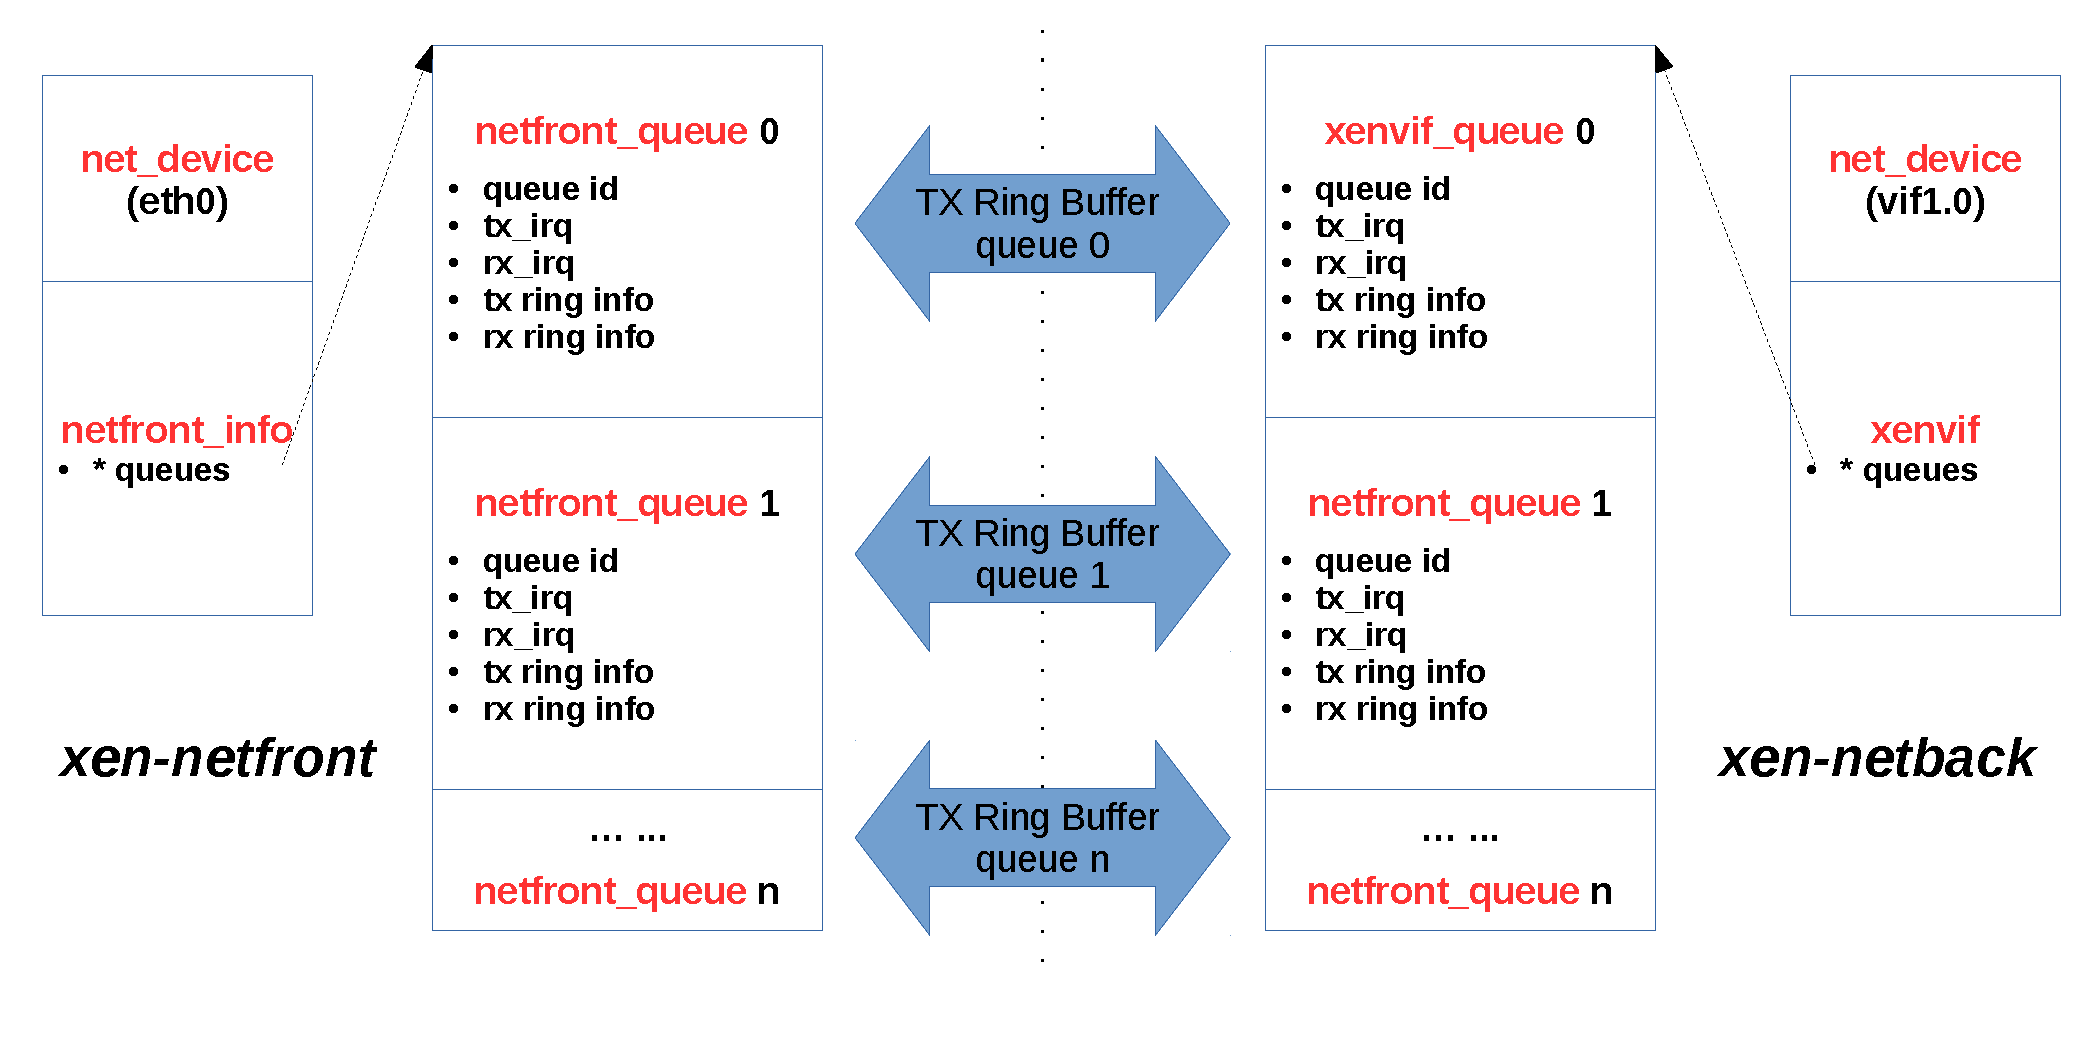
\includegraphics[width=1.0\linewidth]{figures/eth_to_vif.pdf}
\end{figure}
\end{frame}

%------------------------------------------------

\section{pv xmit: front ---> backend 2/3}
\begin{frame}
\frametitle{pv xmit: front ---$>$ backend 2/3}
\begin{figure}
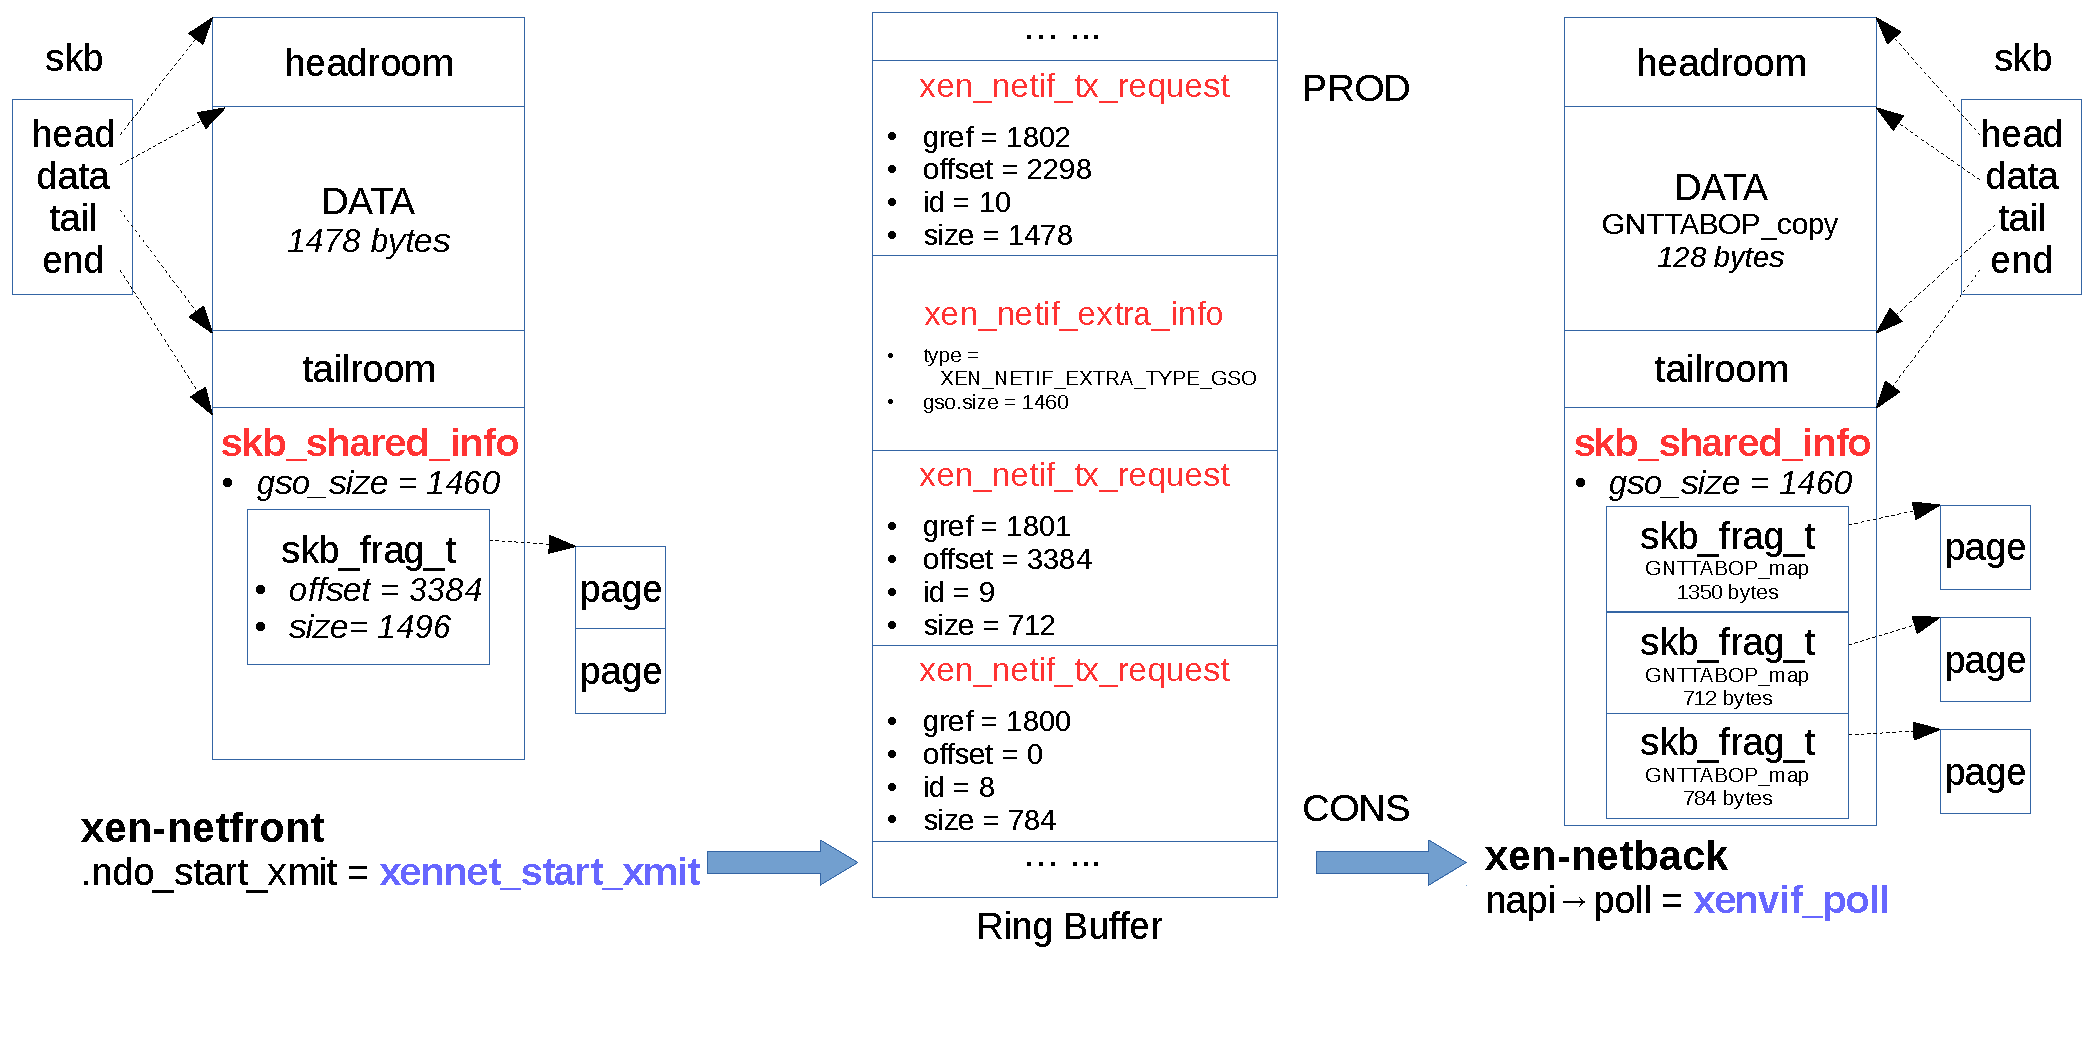
\includegraphics[width=1.0\linewidth]{figures/xmit_skb.pdf}
\end{figure}
\end{frame}

%------------------------------------------------

\section{pv xmit: front ---> backend 3/3}
\begin{frame}
\frametitle{pv xmit: front ---$>$ backend 3/3}
\begin{figure}
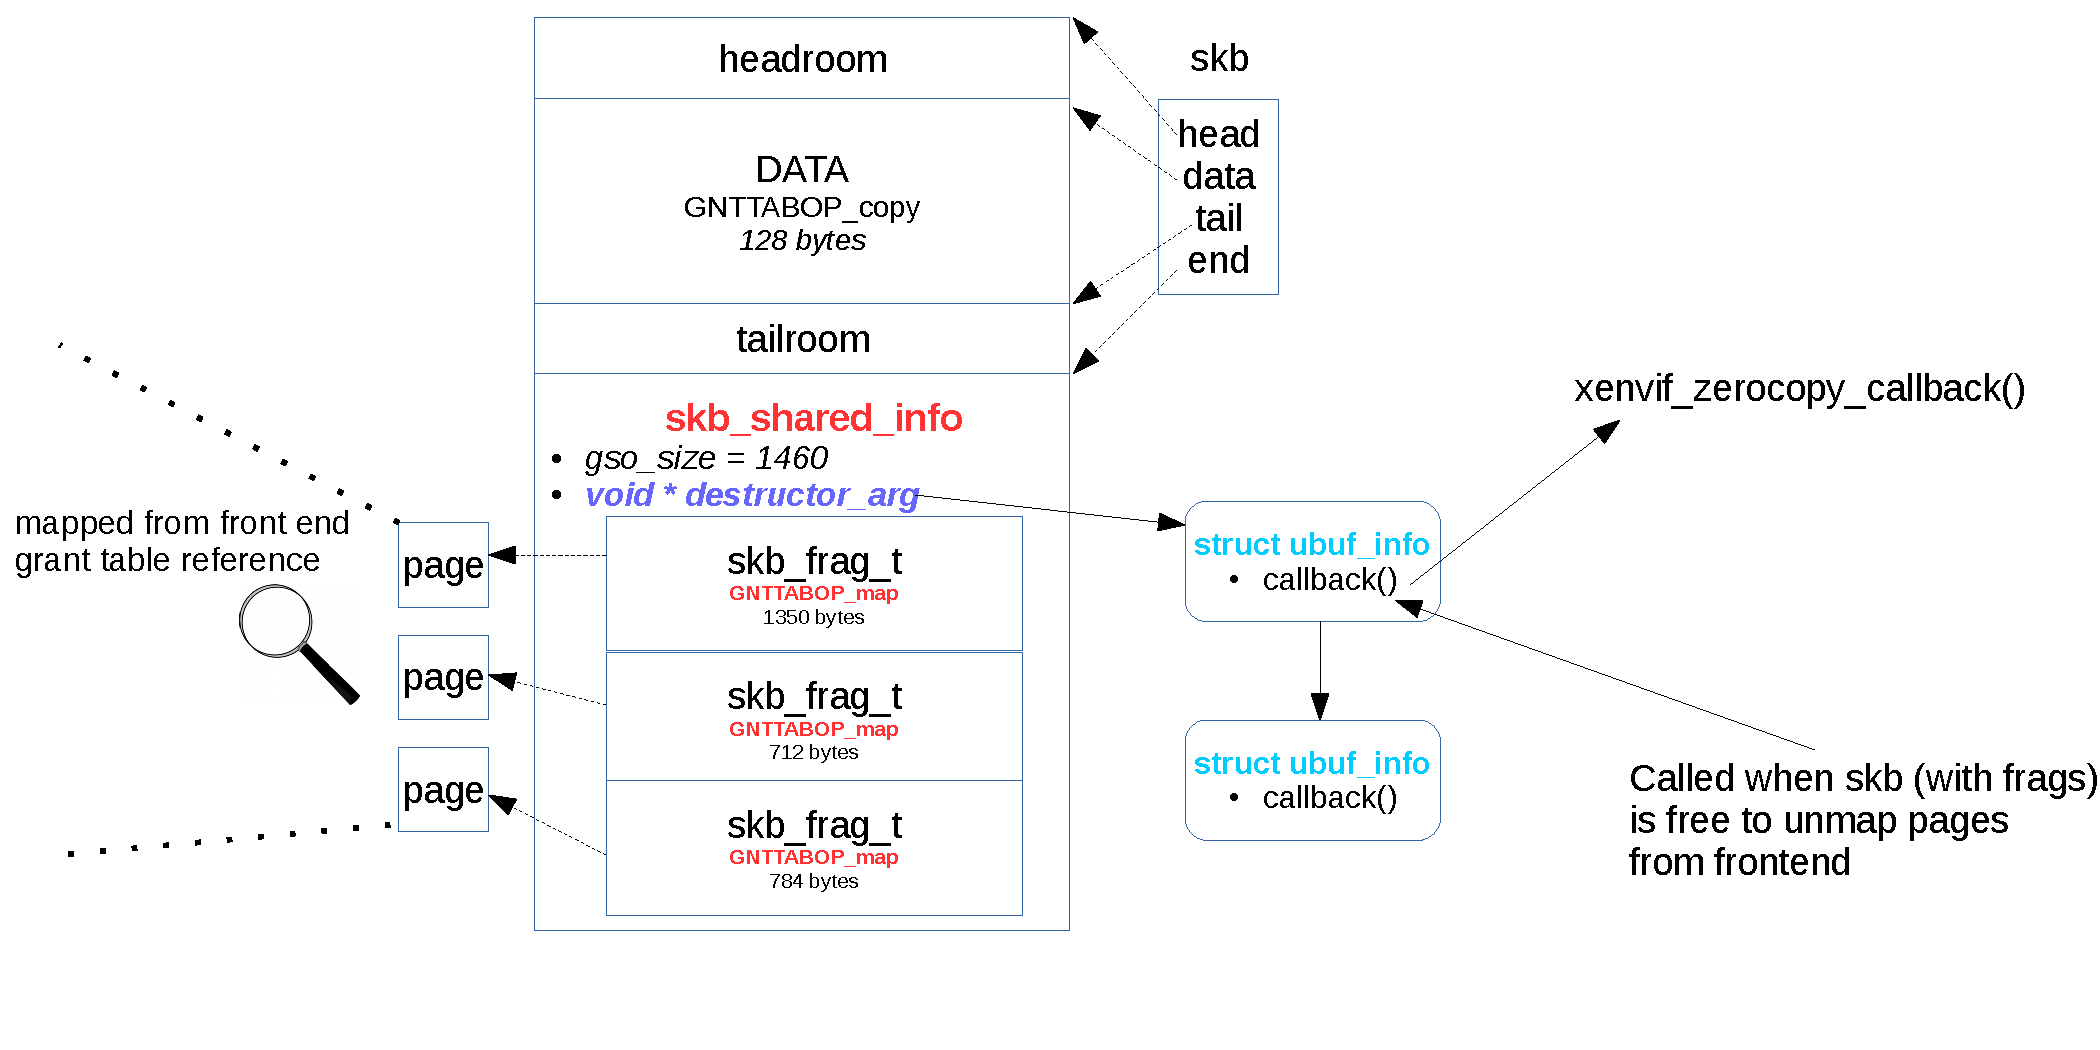
\includegraphics[width=1.0\linewidth]{figures/skb_destruct.pdf}
\end{figure}
\end{frame}

%------------------------------------------------


\section{pv xmit: backend ---> bridge}
\begin{frame}
\frametitle{pv xmit: backend ---$>$ bridge}
\begin{figure}
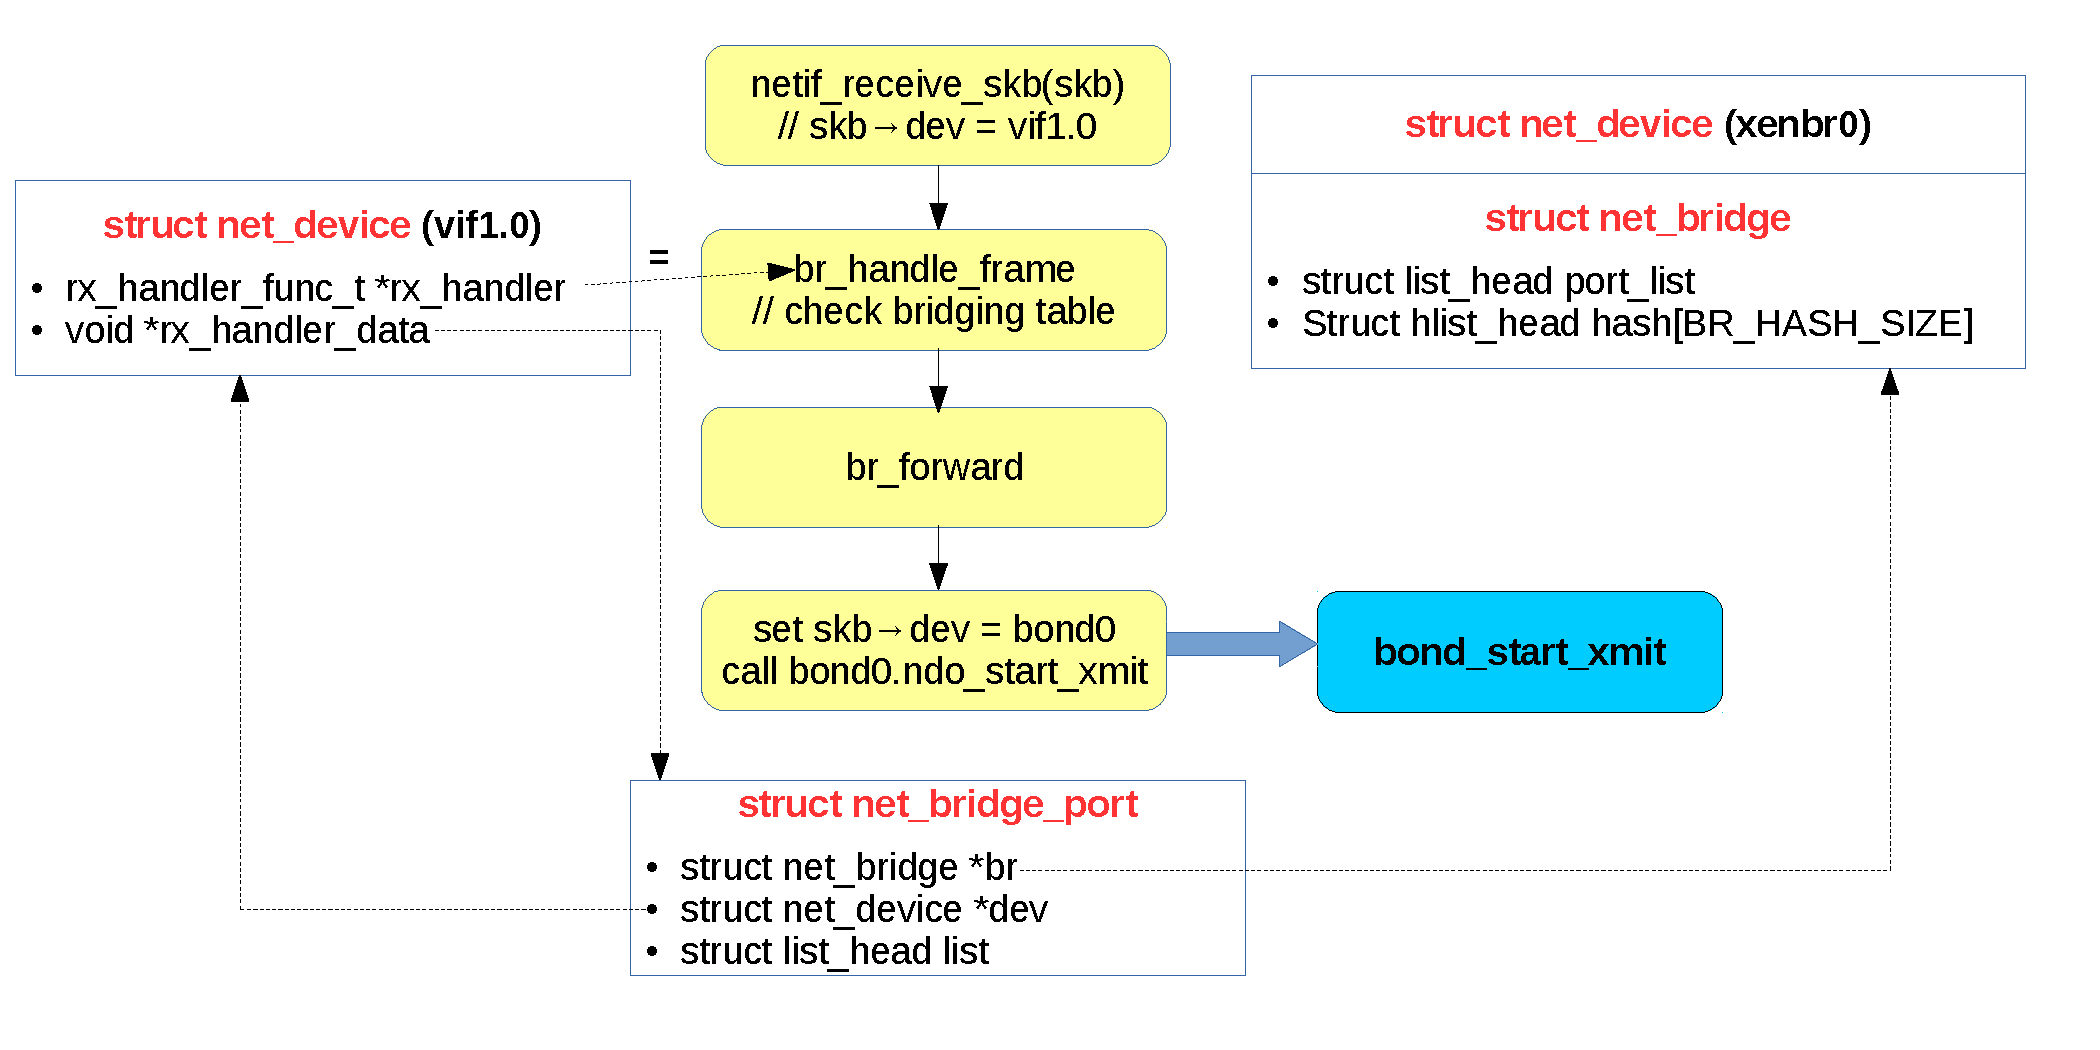
\includegraphics[width=1.0\linewidth]{figures/vif_to_bridge.pdf}
\end{figure}
\end{frame}

%------------------------------------------------

\section{pv xmit: bridge ---> bond ---> physical NIC}
\begin{frame}
\frametitle{pv xmit: bridge ---$>$ bond ---$>$ physical NIC}
\begin{figure}
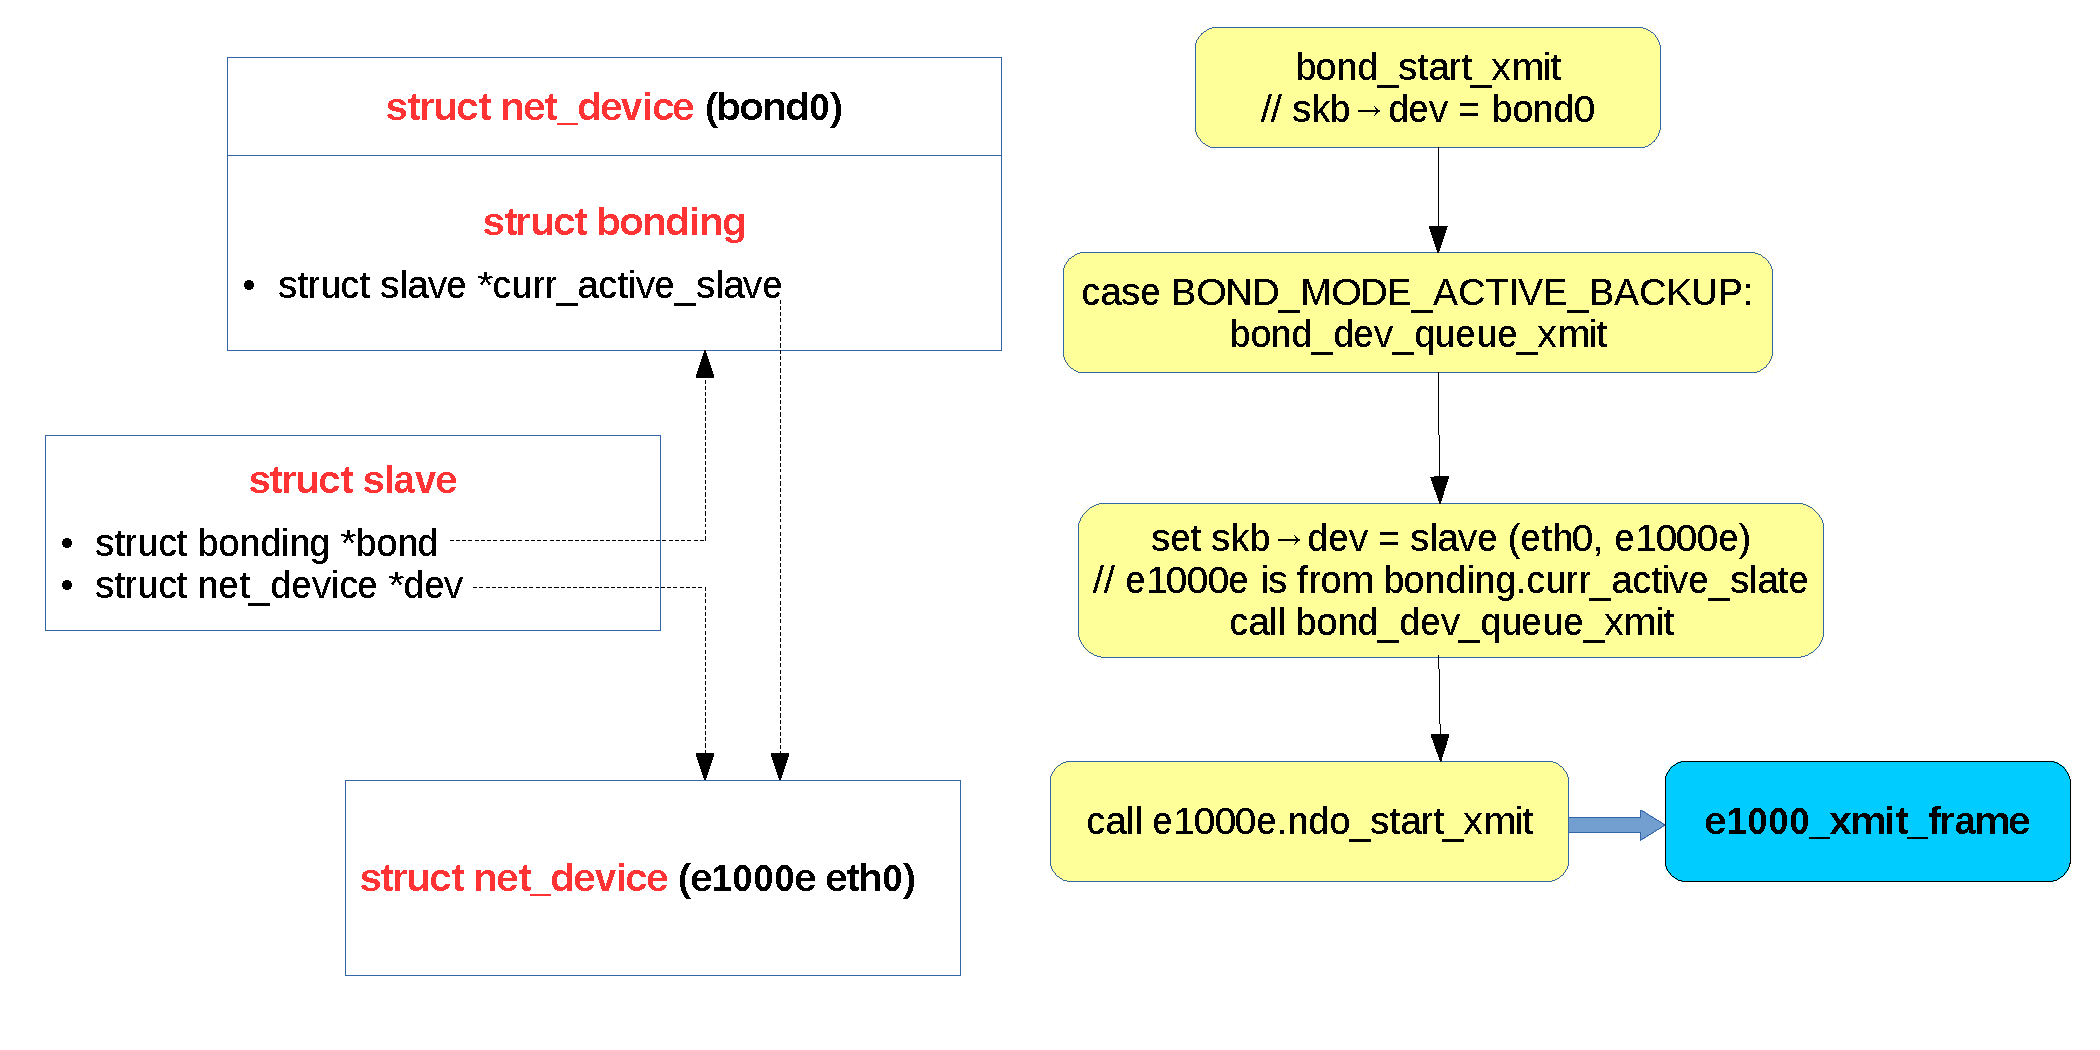
\includegraphics[width=1.0\linewidth]{figures/bridge_to_bond.pdf}
\end{figure}
\end{frame}

%------------------------------------------------

\section{pv recv: physical NIC ---> bond ---> bridge}
\begin{frame}
\frametitle{pv recv: physical NIC ---$>$ bond ---$>$ bridge}
\begin{figure}
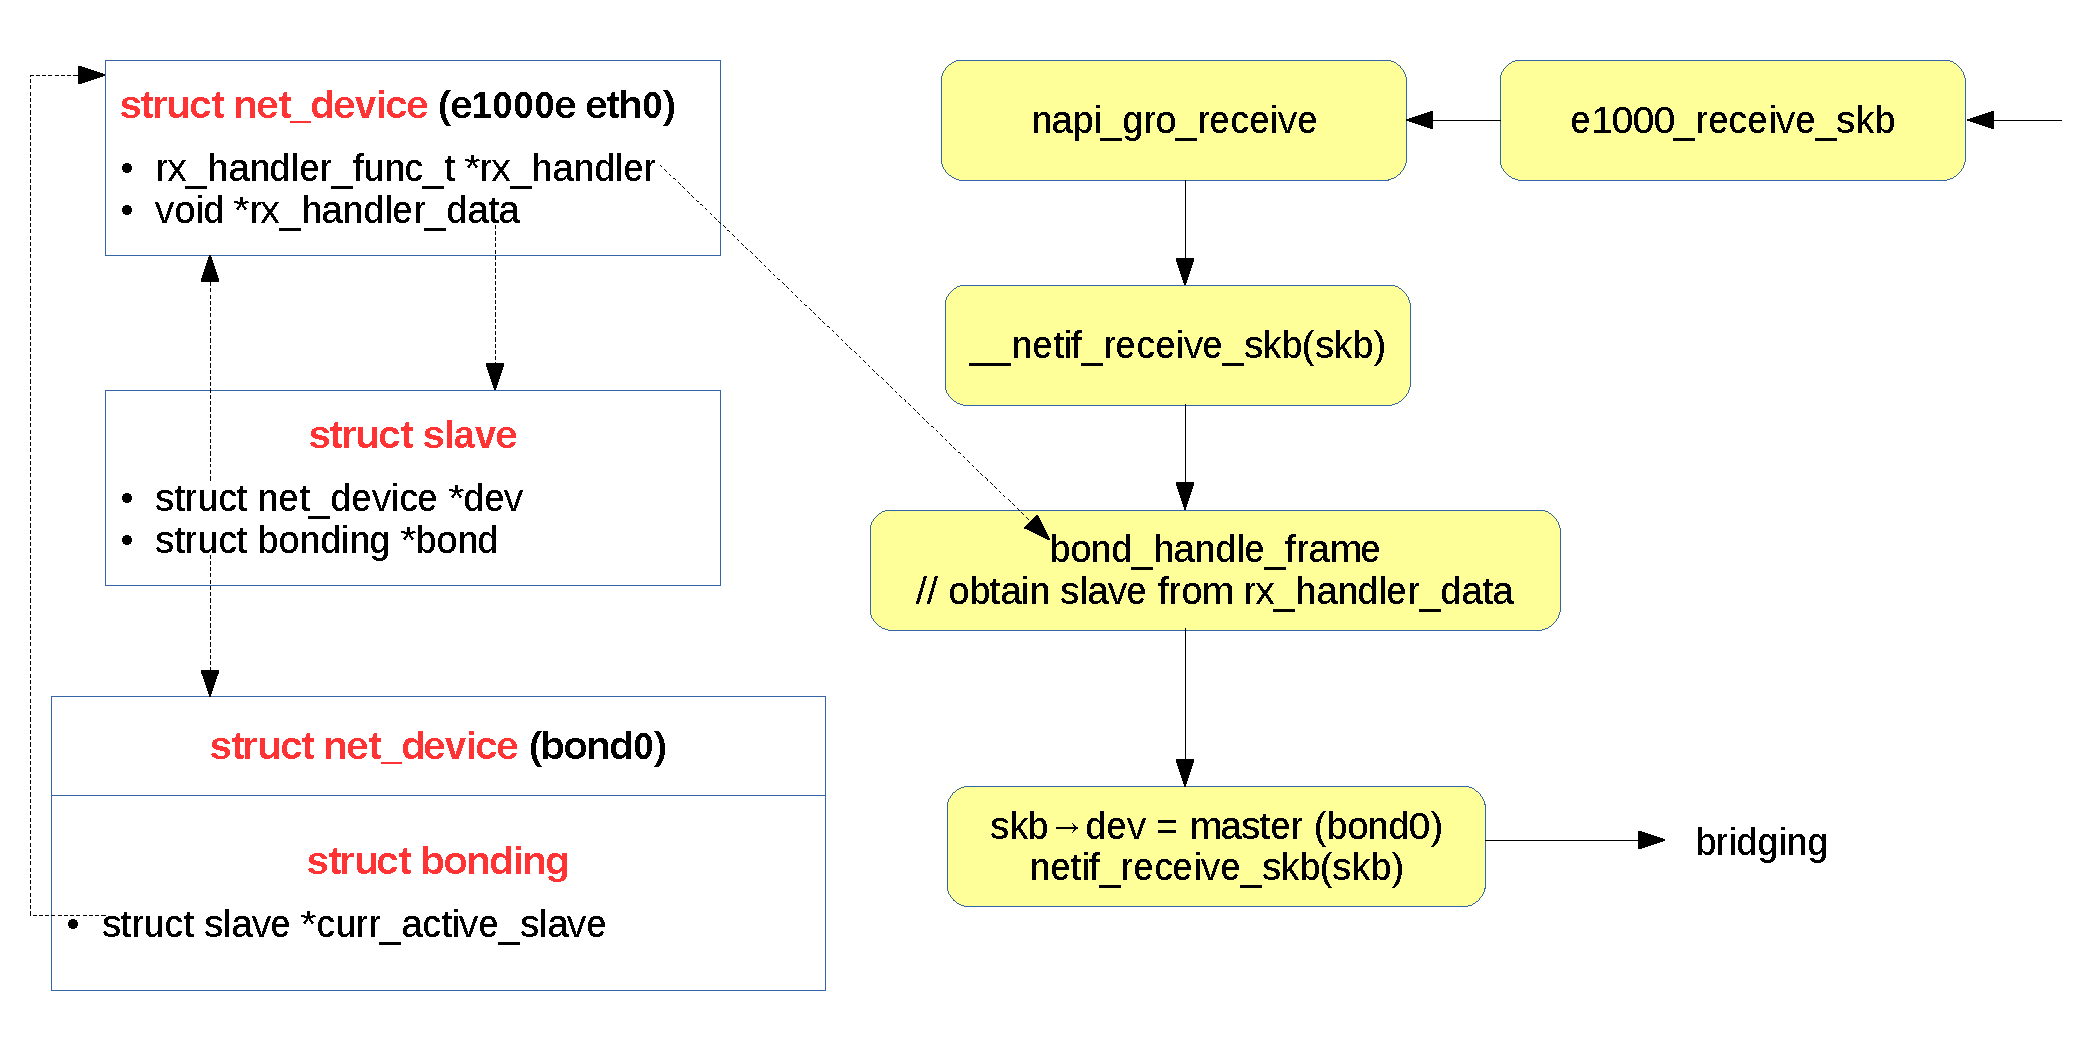
\includegraphics[width=1.0\linewidth]{figures/bond_to_bridge.pdf}
\end{figure}
\end{frame}

%------------------------------------------------

\section{pv recv: bridge ---> backend}
\begin{frame}
\frametitle{pv recv: bridge ---$>$ backend}
\begin{figure}
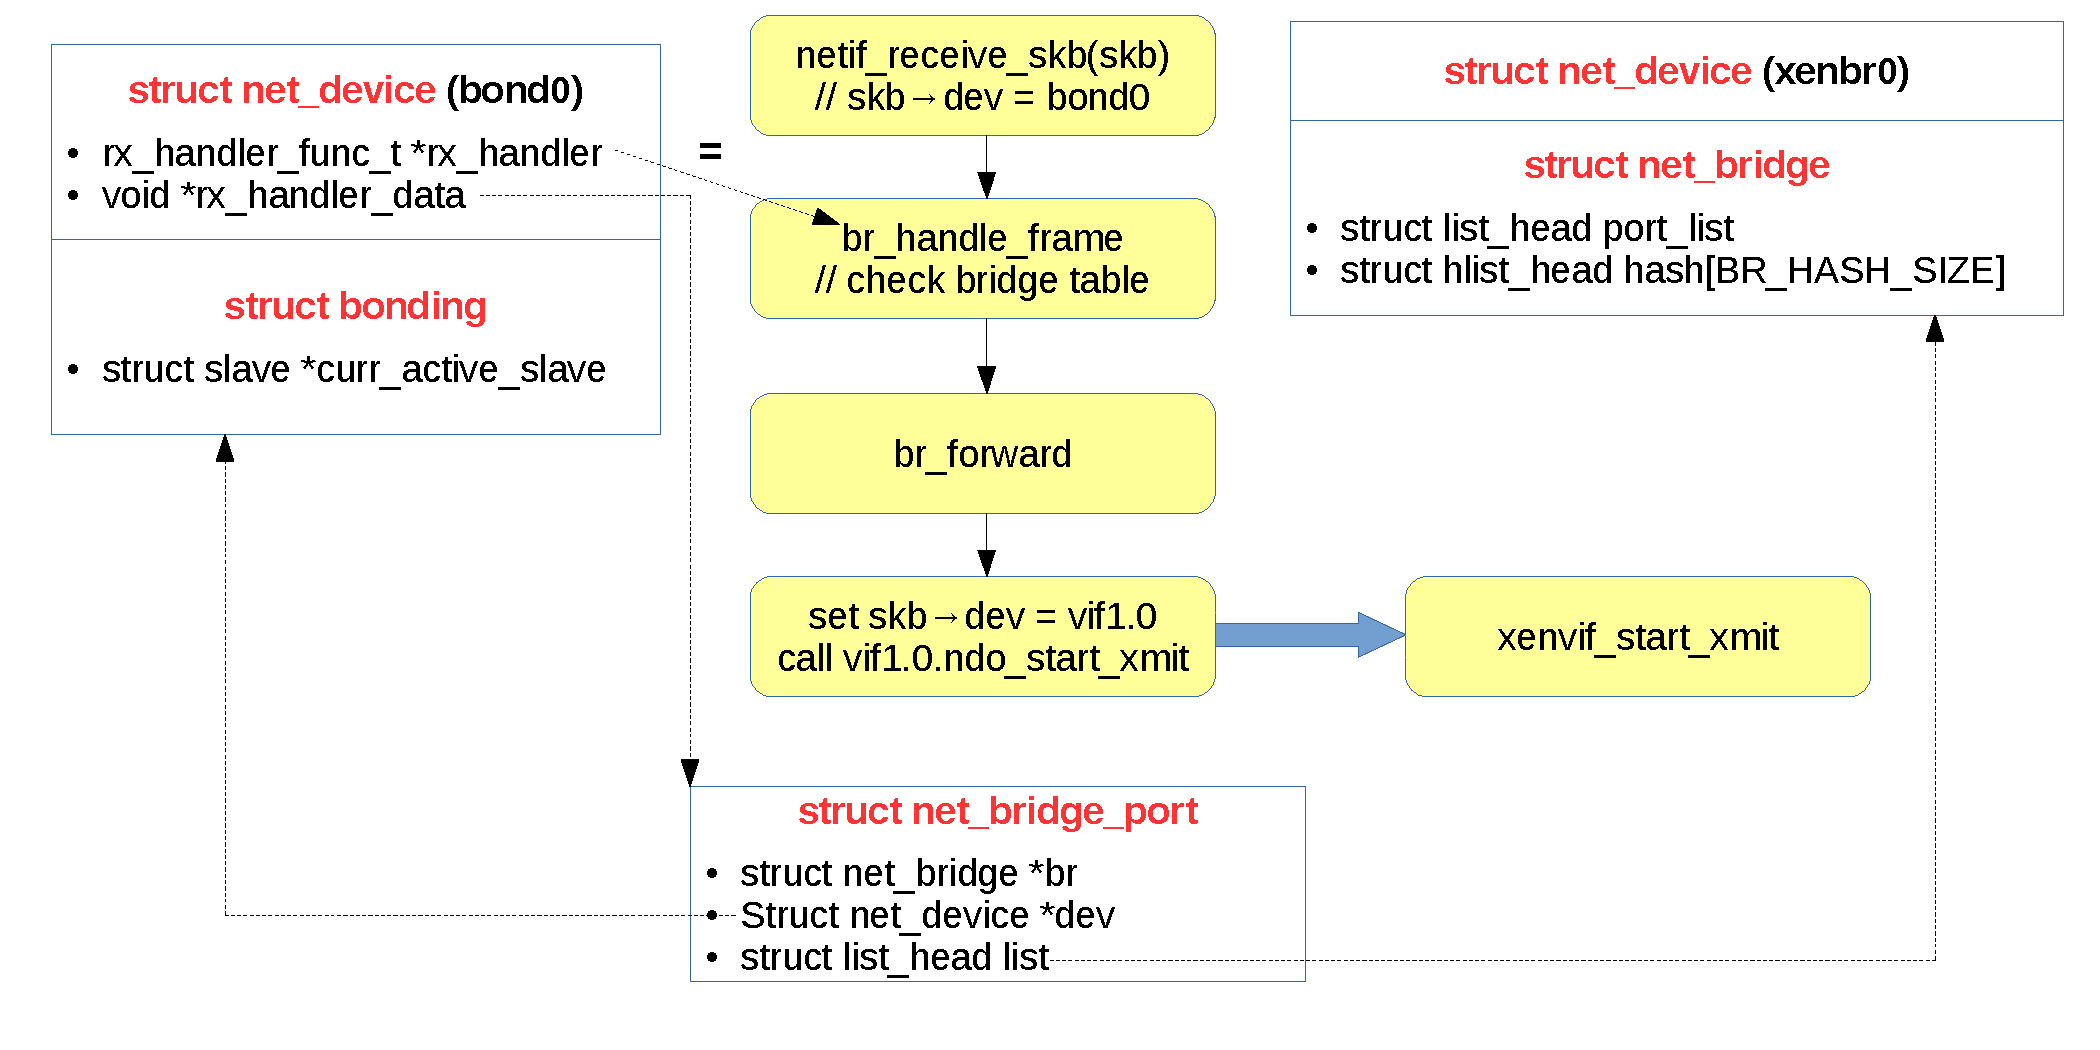
\includegraphics[width=1.0\linewidth]{figures/bridge_to_vif.pdf}
\end{figure}
\end{frame}

%------------------------------------------------

\section{pv recv: backend ---> frontend}
\begin{frame}
\frametitle{pv recv: backend ---$>$ frontend}
\begin{figure}
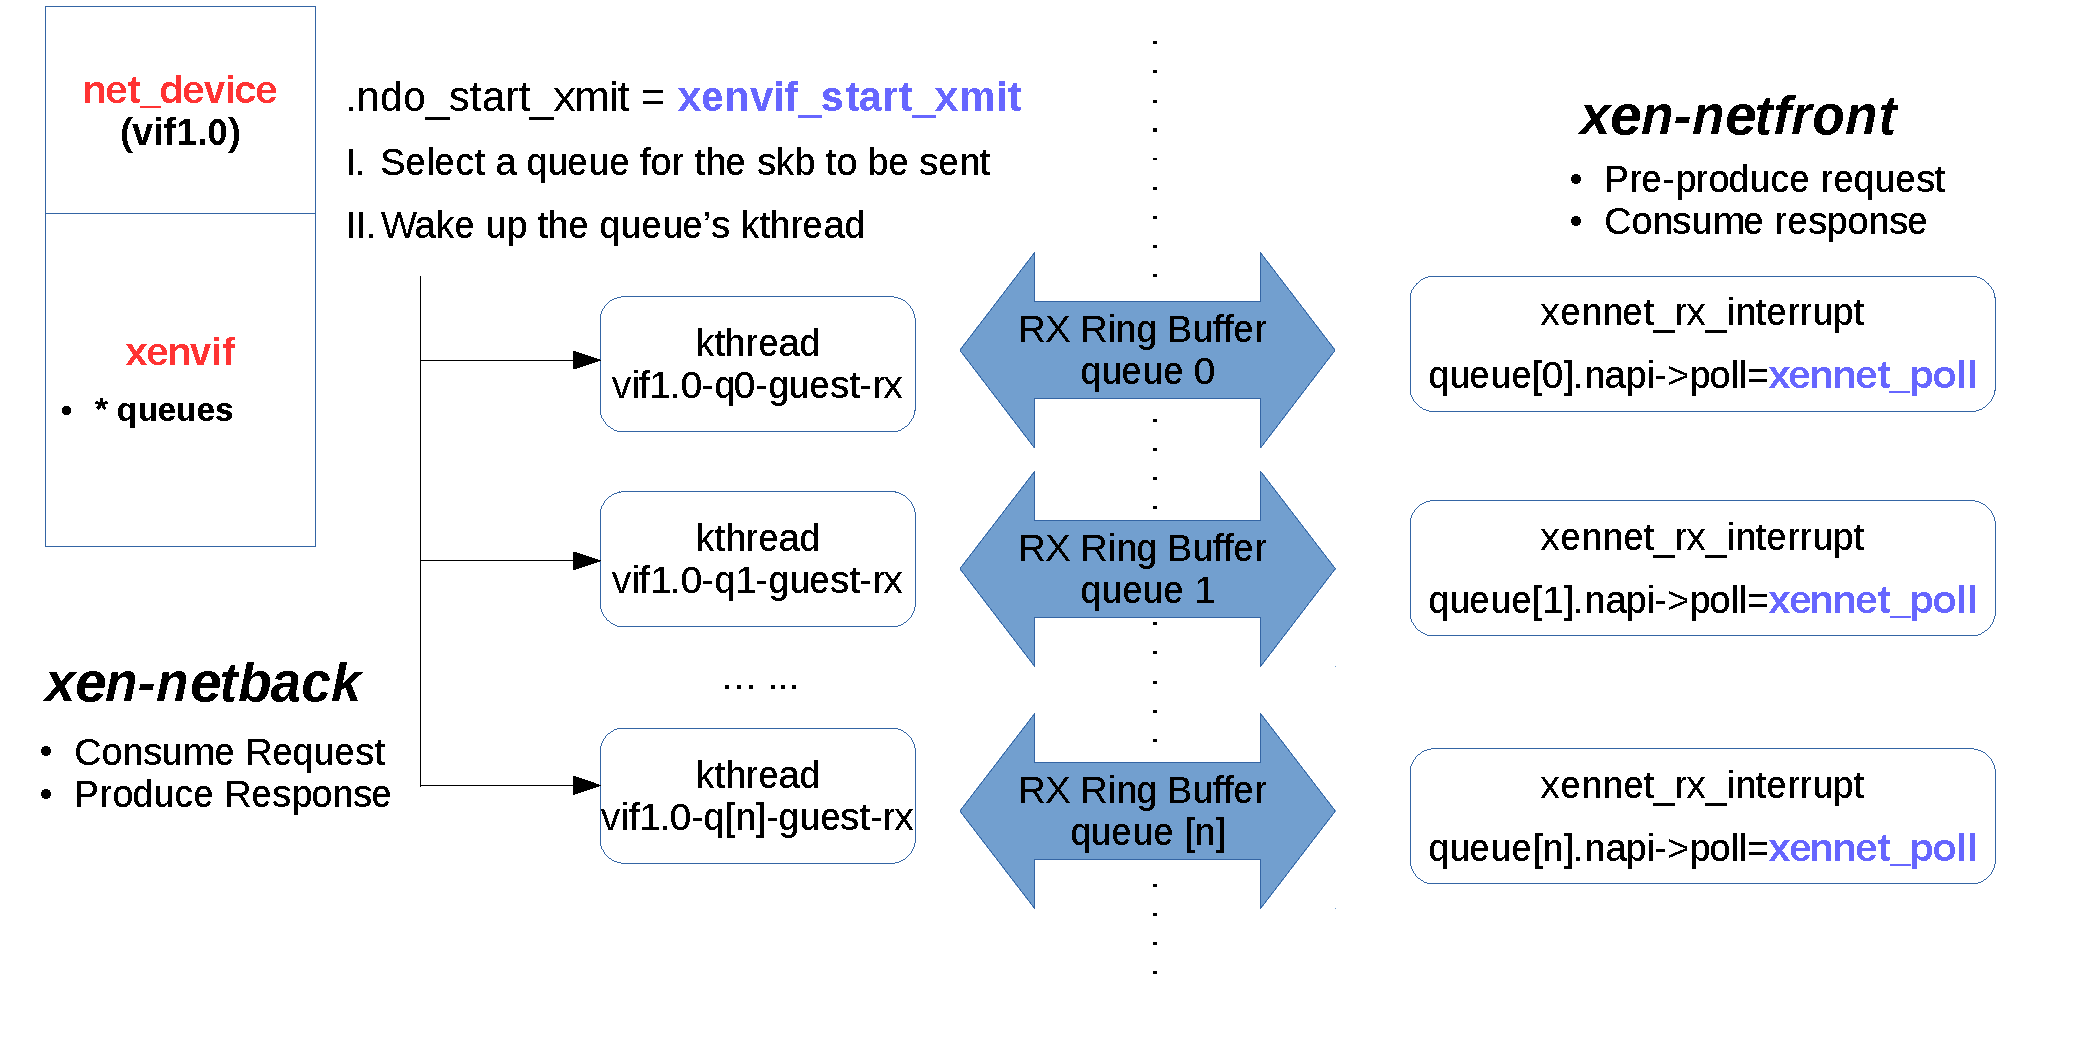
\includegraphics[width=1.0\linewidth]{figures/vif_to_eth.pdf}
\end{figure}
\end{frame}

%------------------------------------------------

\section{xen-netfront/xen-netback summary: req/rsp protocol}
\begin{frame}
\frametitle{xen-netfront/xen-netback summary: req/rsp protocol}
\begin{columns}[c]
\column{.5\textwidth}
\begin{center} \textbf{netfront to netback (produce req)} \end{center}
\begin{enumerate}
\item 1st page of linear data (skb-$>$data)
\item extra info (xen\_netif\_extra\_info)
\item the rest of linear data (skb-$>$data)
\item all skb fragments (skb\_shinfo(skb)-$>$frags)
\end{enumerate}
\column{.5\textwidth}
\begin{center} \textbf{netback to netfront (produce rsq)} \end{center}
\begin{enumerate}
\item 1st page of linear data (skb-$>$data)
\item extra info (xen\_netif\_extra\_info)
\item the rest of linear data (skb-$>$data) 
\item all skb fragments (skb\_shinfo(skb)-$>$frags)
\end{enumerate}
\end{columns}
\end{frame}

%------------------------------------------------

\section{xen-netfront/xen-netback summary: irq and napi}
\begin{frame}
\frametitle{xen-netfront/xen-netback summary: irq and napi}
\begin{figure}
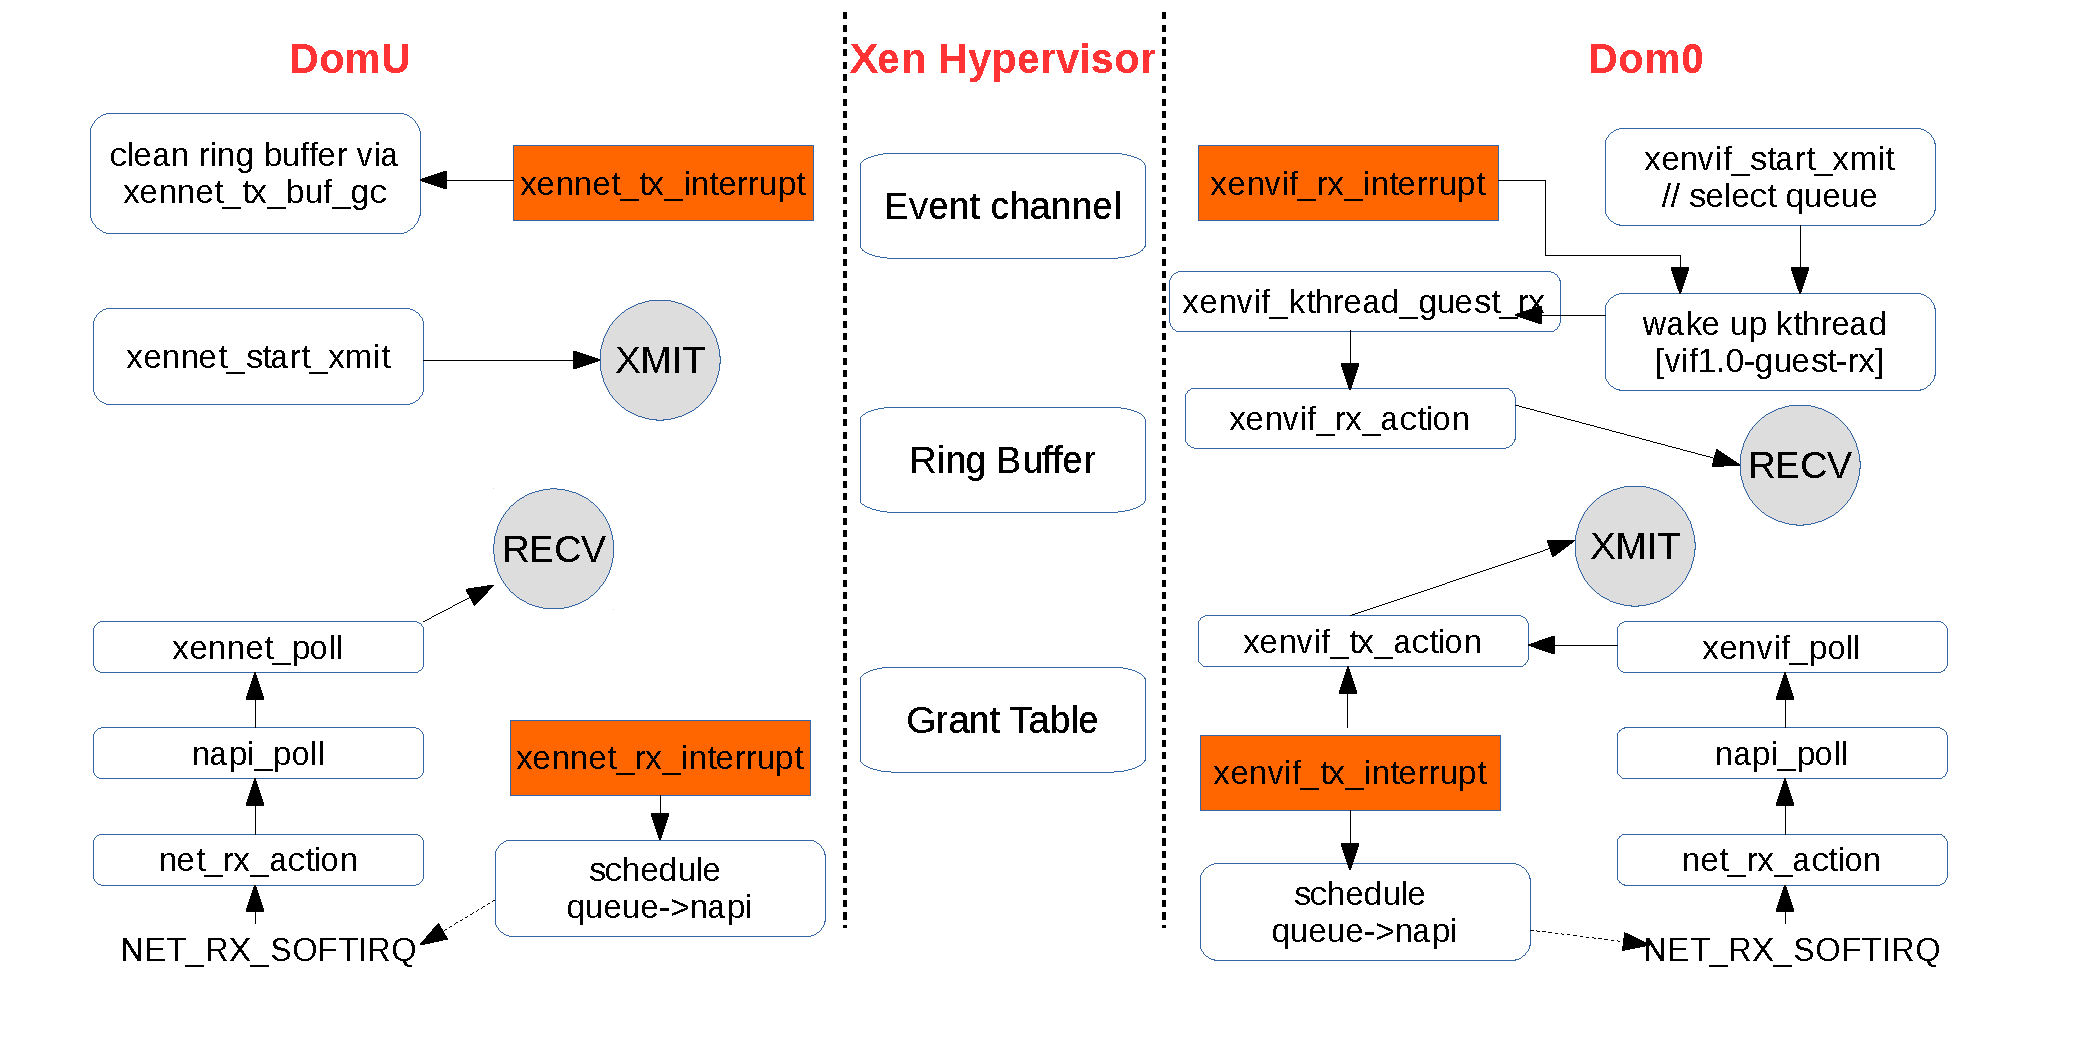
\includegraphics[width=1.0\linewidth]{figures/irq_napi.pdf}
\end{figure}
\end{frame}

%------------------------------------------------

\section{features: multiqueue (default)}
\begin{frame}
\frametitle{features: multiqueue (default)}
\begin{figure}
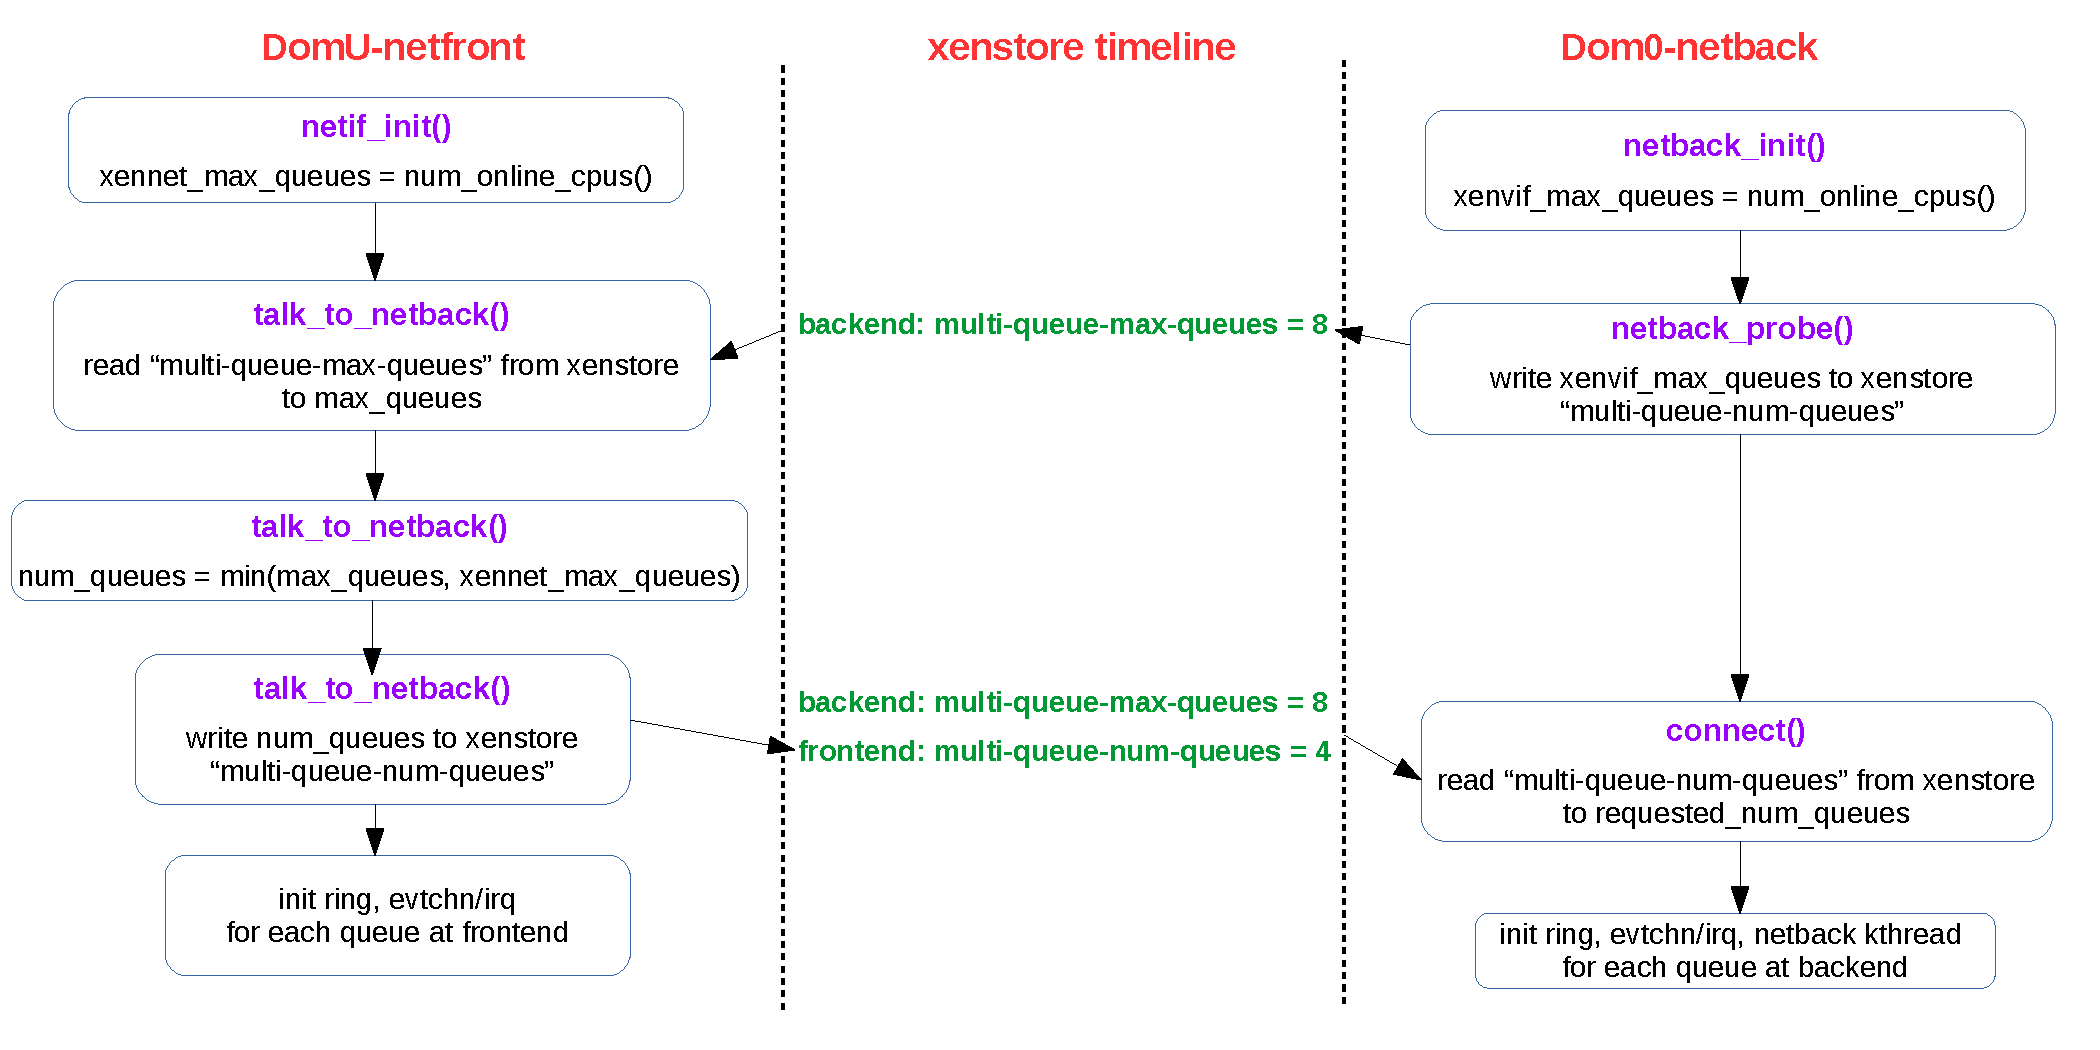
\includegraphics[width=1.0\linewidth]{figures/multiqueue.pdf}
\end{figure}
\end{frame}

%------------------------------------------------

\section{features: gso/tso offload and checksum offload}
\begin{frame}
\frametitle{features: gso/tso offload}
\begin{itemize}
\item {\large Segmentation Offload}
	\begin{itemize}
		\item GSO (Generic Segmentation Offload): software segmentation
		\item TSO (TCP Segmentation Offload): hardware segmentation
	\end{itemize} \pause
\item {\large TSO would postpone segmentation to as late (low level) as possible} \pause
\item {\large TSO info is shared via "struct xen\_netif\_extra\_info gso" in ring buffer}
	\begin{itemize}
		\item gso.gso-$>$u.gso.size = skb\_shinfo(skb)-$>$gso\_size;
		\item gso-$>$u.gso.type = XEN\_NETIF\_GSO\_TYPE\_TCPV6;
	\end{itemize} \pause
\item {\large TSO and other offload features are stored in xenstore (e.g., feature-gso-tcpv4)}
	\begin{itemize}
		\item .ndo\_fix\_features = xennet\_fix\_features
		\item .ndo\_set\_features = xennet\_set\_features
	\end{itemize} \pause
\item {\large checksum offload}
	\begin{itemize}
		\item XEN\_NETTXF\_csum\_blank: Protocol checksum field is blank in the packet (hardware offload)
		\item XEN\_NETTXF\_data\_validated: Packet data has been validated against protocol checksum
	\end{itemize}
\end{itemize}
\end{frame}

%------------------------------------------------

\section{features: multicast}
\begin{frame}
\frametitle{features: multicast}
\begin{figure}
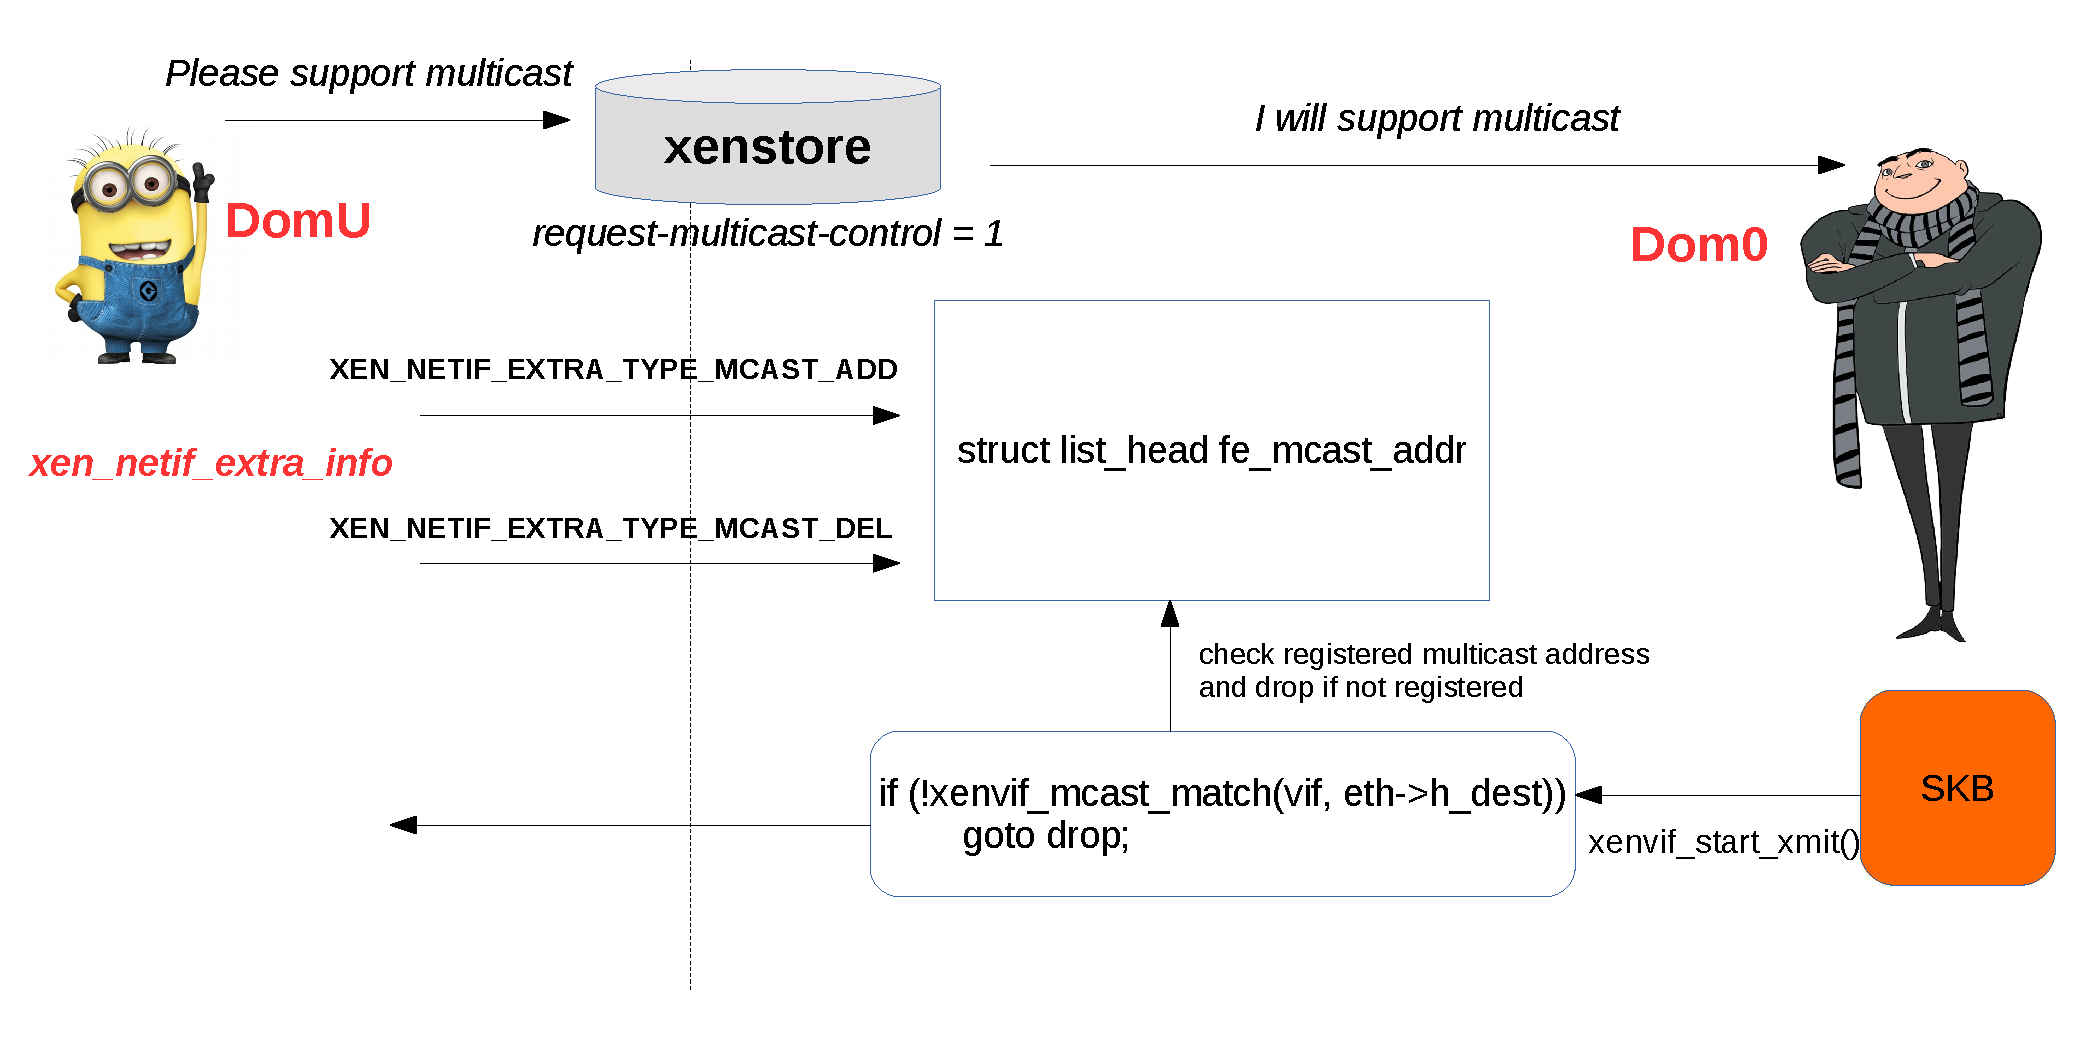
\includegraphics[width=1.0\linewidth]{figures/multicast.pdf}
\end{figure}
\end{frame}

%------------------------------------------------

\section{xen-netfront/xen-netback init}
\begin{frame}
\frametitle{xen-netfront/xen-netback init}
\begin{figure}
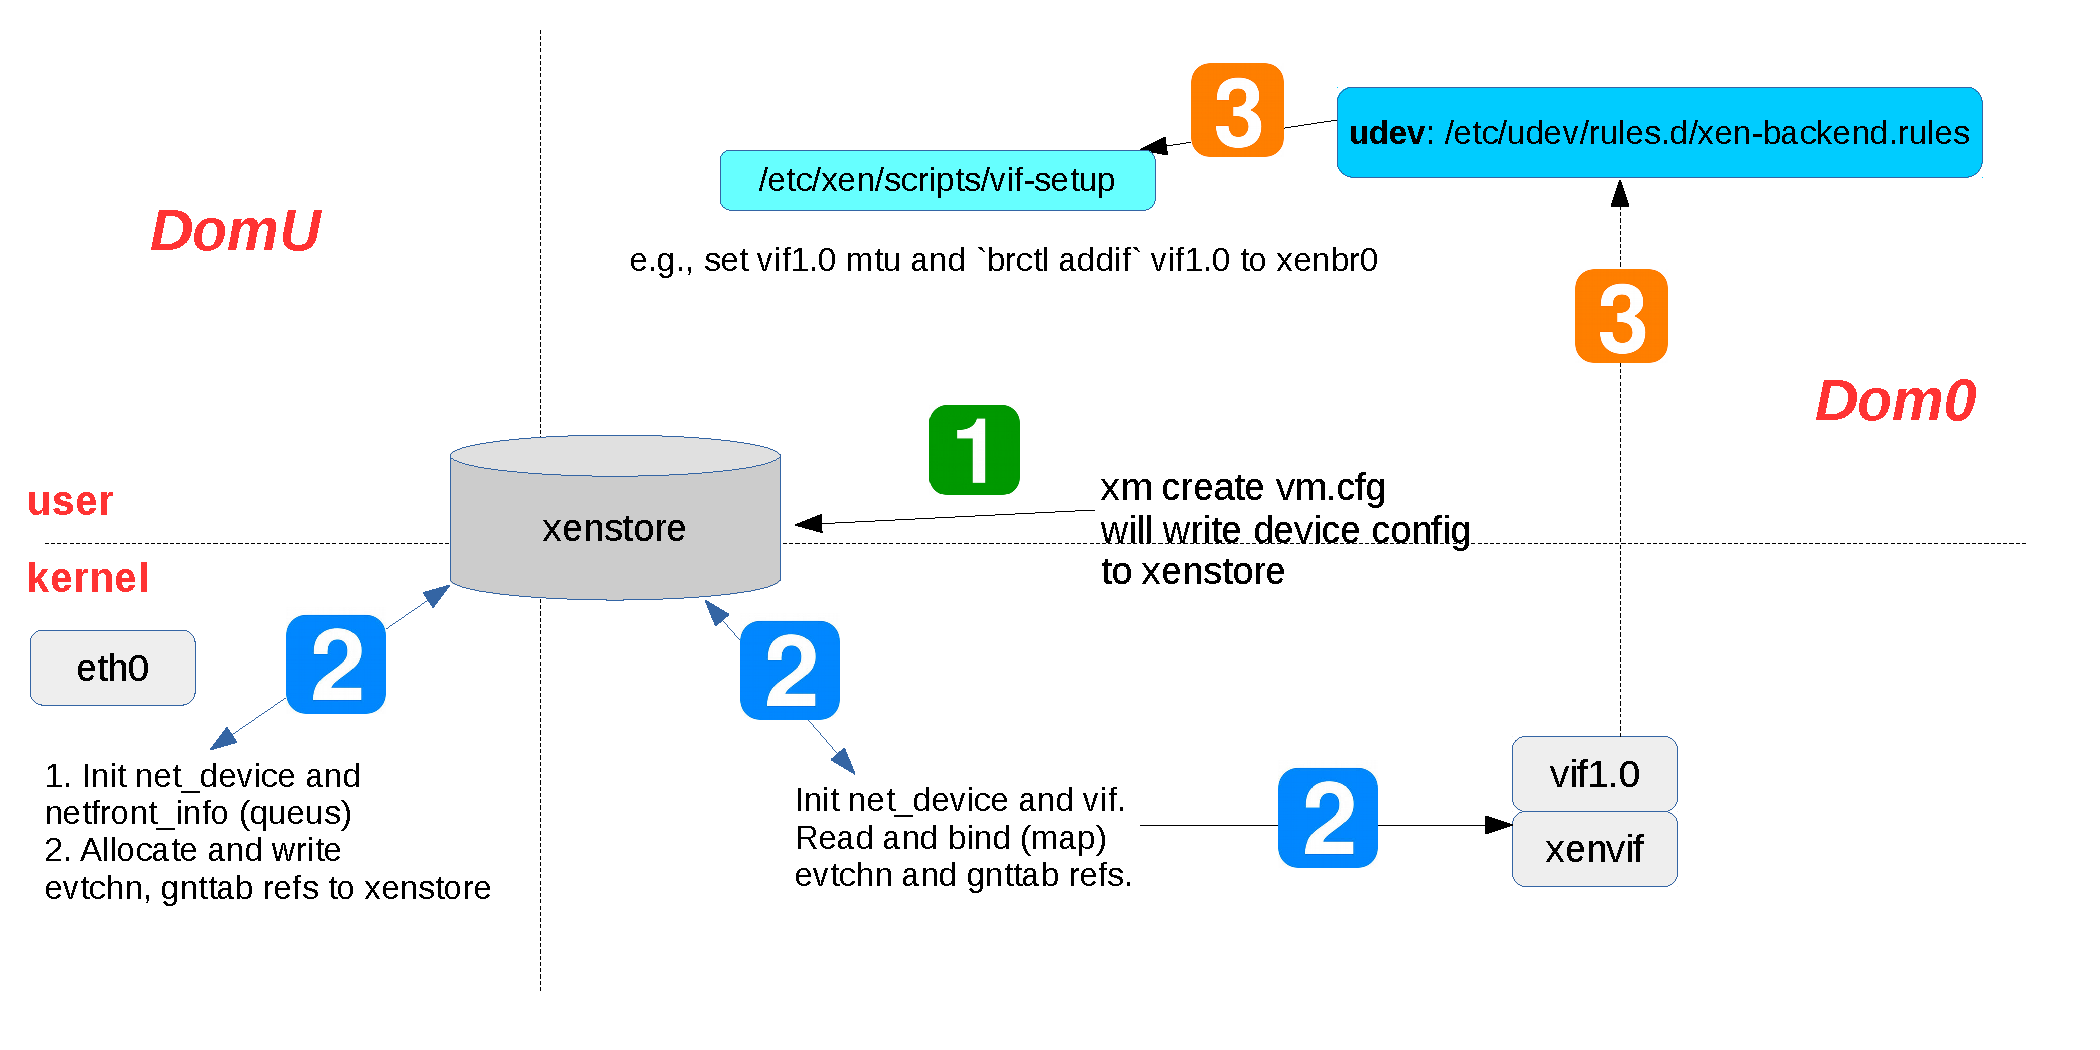
\includegraphics[width=1.0\linewidth]{figures/init.pdf}
\end{figure}
\end{frame}

%------------------------------------------------

\section{performance tuning}
\begin{frame}
\frametitle{performance tuning}
\begin{columns}[c]
\column{.7\textwidth}
\begin{itemize}
\item netfront/netback multiqueue
\item Limit dom0 CPUs to first NUMA socket
\item Interrupt affinity to reduce CPU 0 workload
\item VCPU affinity to improve memory access performance
\item Jumbo frame
\item NIC offload
\item TCP Parameter Settings
\end{itemize}
\column{.3\textwidth}
\begin{center}
\begin{figure}
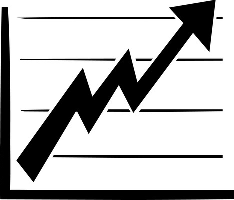
\includegraphics[width=.8\linewidth]{figures/performance.pdf}
\end{figure}
\end{center}
\end{columns}
\end{frame}

%------------------------------------------------

\section{interesting works related to paravirtual I/O}
\begin{frame}
\frametitle{interesting works related to paravirtual I/O}
\begin{itemize}
\item Achieving 10 Gb/s Using Safe and Transparent Network Interface Virtualization. VEE 2009
\item Efficient and Scalable Paravirtual I/O System. USENIX ATC 2013
\item A Comprehensive Implementation and Evaluation of Direct Interrupt Delivery. VEE 2015
\item vRIO: Paravirtual remote I/O.  ASPLOS 2016
\item Hash, don't cache (the page table). SIGMETRICS 2016
\end{itemize}
\end{frame}

%------------------------------------------------

\section{Take-Home Message}
\begin{frame}
\frametitle{Take-Home Message}
\begin{columns}[c]
\column{.7\textwidth}
\begin{itemize}
\visible<1->{\item Xen paravirtual networking workflow}
\visible<2->{\item Xen paravirtual networking framework}
\visible<3->{\item Xen paravirtual networking init, protocol, features}
\visible<4->{\item Xen paravirtual networking performance}
\end{itemize}
\column{.3\textwidth}
\begin{center}
\begin{figure}

\includegraphics[width=.8\linewidth]{figures/home.pdf}
\end{figure}
\end{center}
\end{columns}
\end{frame}

%\begin{frame}
%\Huge{\centerline{The End}}
%\end{frame}

%----------------------------------------------------------------------------------------

\end{document} 
